\documentclass[11pt]{article}
\usepackage[review]{acl}
\usepackage{times}
\usepackage{latexsym}
\usepackage[T1]{fontenc}
\usepackage[utf8]{inputenc}
\usepackage{microtype}
\usepackage{inconsolata}
\usepackage{amssymb}
\usepackage{graphicx}
\graphicspath{{results/}}
\usepackage{multicol}
\usepackage{amsmath}
\usepackage{dsfont}
\usepackage{float}
\usepackage{subcaption}
\usepackage{xcolor}
\usepackage{booktabs}
\usepackage{multirow}

% Loosen float placement so figures aren't deferred to end of document
\renewcommand{\topfraction}{0.9}
\renewcommand{\textfraction}{0.1}
\renewcommand{\floatpagefraction}{0.85}
\setcounter{topnumber}{4}
\setcounter{dbltopnumber}{4}

\title{Empirical Verification of Linear Task Superposition in LLMs}

\author{Anonymous}

\begin{document}

\maketitle

\begin{abstract}
When in-context examples span multiple tasks, LLMs have been shown to represent and perform all of them simultaneously in a phenomenon called task superposition. Although previous work posits a convex combination of individual task vectors for this superposition, there is no thorough empirical verification of this hypothesis in deployed LLMs. In this study, we explore the representations with mixed task prompts, empirically verifying linearity in task superposition. This is shown across different model families and scales, as well as task groups, highlighting that linearity is indeed a generalizable property for how task vectors superpose. We also quantify linear superposition fidelity via a normalized projection of the actual mixed-task centroid onto the linearly predicted position. We further exploit this linearity to recover task mixture coefficients via reparametrized OLS, and show that the true mixture ratios fall within the 95\% bootstrap confidence intervals of the recovered estimates in 9 of 10 tested conditions.
\end{abstract}

\section{Introduction}
In-context learning (ICL) enables large language models to adapt to new tasks from only a handful of demonstrations, without updating model parameters \citep{brown2020language}. Understanding how transformers internally represent these inferred tasks has become a central question in mechanistic interpretability. Recent work has shown that in-context learning induces latent task representations, or task vectors, within transformer hidden states \citep{Hendel2023-yk, Dong2025-jo}. Building on this perspective, \citet{xiong2024oncellmsincontextlearn} introduced task superposition, hypothesizing that mixed-task prompts produce representations that are linear combinations of individual task vectors. While this hypothesis is supported by behavioral evidence and visualization, it has not been directly evaluated at the representational level.\\[1em]
Verifying the geometry of task representations is important for understanding how transformers internally encode and combine multiple tasks. Although recent work has proposed linear models of task representations and observed behavioral evidence consistent with task superposition, it remains unclear whether these hypotheses accurately describe the hidden representations of modern instruction-tuned language models. Additionally, it poses implications for representation steering for predictably altering model behavior. \\[1em]
In this work, we make the following contributions:
\begin{itemize}
    \item We directly analyze task vector superposition at a representational level, showing that the linear relationship of task vectors holds when in-context examples from multiple tasks are mixed. This phenomenon is tested across multiple task groups, as well as different instruct-tuned model families and scales.
        \item To further validate this linearity, we demonstrate that the true mixture ratios lie within a 95\% confidence interval of the estimated coefficients through re-parameterized OLS, which are estimated without any prior knowledge of the task distribution in the context examples.
    \item To account for the effect of test questions, we use contrast vectors instead of task vectors, subtracting the assistant header activations in prompts with just the test question from the activations in prompts with the in-context examples along with the test question.
\end{itemize}

\section{Related work}
\subsection*{Task Vector Geometry in In-Context Learning}
Recent work has characterized in-context learning through the lens of task vectors- latent vector representations in the transformer's residual stream that summarize the task specified by a set of in-context demonstrations. \citet{Hendel2023-yk} introduce the task vector \(\theta(S)\), derived from in-context examples \(S\), and show that it captures the task-relevant information necessary for in-context learning. They show that with a test question \(x\), a function \(f(x, \theta)\) using the extracted task vector closely reproduces the behavior of the original transformer conditioned on the in-context demonstrations \(S\). This suggests that task vectors provide a compact representation of the task inferred from the demonstrations. \\[1em]
\citet{Dong2025-jo} build on this perspective by proposing the \textit{Linear Combination Conjecture}, positing that task vectors function as a compressed representation of in-context demonstrations formed through linear combinations of the original examples provided in the prompt. Extending this idea, \citet{yan2026taskvectorgeometryunderlies} provide a theoretical characterization of task-vector geometry in a controlled pretraining setting, modeling hidden representations as convex combinations of learned task vectors weighted by the posterior probability of each latent task. Under this framework, in-distribution task inference corresponds to Bayesian retrieval over previously learned tasks, with the mixture coefficients reflecting the model’s inferred task distribution. Together, these works suggest that task information is encoded within a structured linear latent space, providing theoretical motivation for investigating whether analogous linear task composition emerges in instruction-tuned language models during in-context learning. \\[1em]
While these works focus on representations induced by a single task, \citet{xiong2024oncellmsincontextlearn} extend this perspective to prompts containing demonstrations from multiple tasks. They introduce task superposition- the ability of LLMs to perform distinct tasks simultaneously. They investigate the presence of this phenomenon during both training and inference times, across different model families and scales, and for different task groups, analyzing the top K probability distribution of gold answer tokens. They also view task superposition through the lens of task vectors, using LDA projection to observe the relation between the mixing ratio of tasks in the ICL prompt and the location of the task vectors in LDA space. This notion of task superposition is complementary to recent theoretical work on task-vector geometry, which models in-distribution task inference through convex combinations of latent task vectors \citep{yan2026taskvectorgeometryunderlies}. \\[1em]
We build on this work by testing for linear superposition at the representational level across various model families and task groups. This is tested in finetuned models (unlike \citet{xiong2024oncellmsincontextlearn}, who tested this phenomenon on pretrained models). We also demonstrate a framework for recovering the mixture ratio of in-context examples using precomputed contrast vectors for individual tasks.
\subsection*{Representation Decomposition and Shared Features}
\subsection*{Notions of Superposition}
The term superposition has been used in multiple contexts within deep learning. In mechanistic interpretability, feature superposition refers to the phenomenon where individual neurons encode multiple unrelated features due to representational compression \citep{elhage2022toymodelssuperposition}. In this work, we instead adopt the notion of task superposition introduced by \citet{xiong2024oncellmsincontextlearn}- the ability of a model to perform multiple tasks given in-context examples of those tasks in a single forward pass. Although these notions operate at different levels of abstraction, both describe multiple entities sharing a common latent representation.

\section{Experimental Setup}
In this section, we discuss the core setup for the experiments which will follow. We will explicitly define the aforementioned contrast vector and also discuss the metric \(\kappa\) used to quantify the extent to which linearity holds.
\subsection{Task groups}
\label{subsec:taskgrps}
We consider three task groups--- Arithmetic addition, Entity attribution to countries, and multiple choice questions from Massive Multitask Language Understanding (MMLU) \citep{Hendrycks2020-ae}. \\[1em]
\textbf{Arithmetic tasks}--- these tasks are intended to analyze contrast vector representations when the formats of the in-context examples are varied while preserving semantic content (arithmetic addition) across tasks. Two integers \texttt{op1} and \texttt{op2} are randomly generated and used to generate addition questions in one of 3 formats:
\begin{itemize}
    \item Direct--- this task requires reporting the direct addition computation in numerical format.
    \item Multiple Choice--- this task requires reporting the multiple choice option corresponding to the correct answer of the addition. Each question has 4 options labeled A-D. To control for the effects of distractor options in affecting the question format within a single task, we keep the distractors at a maximum offset of \(\pm 10\) from the true answer.
    \item Verification--- this task requires reporting a ``yes'' or ``no'' based on if the proposed answer to the addition problem is indeed correct. Again, to control for the effects of the potential answer affecting the question format, we offset the true sum by a maximum of \(\pm 3\) to generate incorrect answers.
\end{itemize}
In all three tasks, the \texttt{A:} token is used as an answer prompt to isolate format differences to the question rather than the output trigger. The multiple choice task has a wider maximum offset while the verification has a smaller offset, both of which provide more plausible distractors for their respective tasks. \\[1em]
\textbf{Entity tasks}-- these tasks focus on semantic relation. The tasks in this group involve mapping a country to its capital, currency, and language from a manually constructed dataset. Unlike the other task groups, we do not use any assistant trigger for this task group in the user prompts.\\[1em] 
\textbf{MMLU tasks}--- these tasks are intended to analyze contrast vector representations when the semantic nature of the in-context examples are varied while preserving question format across tasks. Multiple choice questions randomly sampled from the MMLU dataset from the World History, Law, and Machine Learning domains are used in this task group, all in the same format. \\[1em]
In all three tasks, \texttt{Answer:} is used as an answer prompt to elicit a single-letter response while holding the prompt format constant. By restricting ourselves to multiple choice questions, we ensure that the separation and task superposition seen in projected contrast vectors is due to variations in semantics, not syntax/format. Prompt formats for all task groups are shown in \autoref{tab:prompt_formats}. Further implementation details on sampling for each task group are provided in \autoref{appendix:sampling}.

\begin{table*}[t]
\centering
\small
\renewcommand{\arraystretch}{1.4}
\caption{Prompt formats for each task and task group.}
\label{tab:prompt_formats}
\begin{tabular}{llp{0.42\textwidth}p{0.28\textwidth}}
\toprule
\textbf{Group} & \textbf{Task} & \textbf{In-context Example} & \textbf{Test Question} \\
\midrule
\multirow{3}{*}{Arithmetic}
  & Direct
  & \texttt{User: \{op1\} + \{op2\} A:}\newline\texttt{Assistant: \{op1+op2\}}
  & \texttt{User: \{op1\} + \{op2\} A:} \\[3ex]
  & MCQ
  & \texttt{User: \{op1\}+\{op2\}=?}\newline\texttt{A) \{optA\} B) \{optB\}}\newline\texttt{C) \{optC\} D) \{optD\} A:}\newline\texttt{Assistant: B}
  & \texttt{User: \{op1\}+\{op2\}=?}\newline\texttt{A) \{optA\} B) \{optB\}}\newline\texttt{C) \{optC\} D) \{optD\} A:} \\[3ex]
  & Verification
  & \texttt{User: \{op1\}+\{op2\}=x.}\newline\texttt{Correct? A:}\newline\texttt{Assistant: yes/no}
  & \texttt{User: \{op1\}+\{op2\}=x.}\newline\texttt{Correct? A:} \\
\midrule
\multirow{3}{*}{Entity}
    & Capital
    & \texttt{User: \{country\}}\newline\texttt{Assistant: capital[\{country\}]} & \texttt{User: \{country\}} \\[3ex]
    & Currency
    & \texttt{User: \{country\}}\newline\texttt{Assistant: currency[\{country\}]} & \texttt{User: \{country\}} \\[3ex]
    & Language 
    & \texttt{User: \{country\}}\newline\texttt{Assistant: language[\{country\}]} & \texttt{User: \{country\}} \\
\midrule
MMLU & History/Law/ML
  & \texttt{User: Question: \{question\}}\newline\texttt{A) \{optA\} B) \{optB\}}\newline\texttt{C) \{optC\} D) \{optD\}}\newline\texttt{Answer:}\newline\texttt{Assistant: B}
  & \texttt{User: Question: \{question\}}\newline\texttt{A) \{optA\} B) \{optB\}}\newline\texttt{C) \{optC\} D) \{optD\}}\newline\texttt{Answer:} \\
\bottomrule
\end{tabular}
\end{table*}

\subsection{In-context example ratios}
\label{subsec:icl_ratios}
All prompts contain 3 in context examples and 1 test question. For the 3 in-context examples, we vary the tasks they correspond to. For all three task groups, we consider the following 10 ratios of tasks:
\begin{itemize}
    \item Pure ratios: (3, 0, 0), (0, 3, 0), (0, 0, 3)
    \item Mixed ratios: (2, 1, 0), (1, 2, 0), (0, 2, 1), (0, 1, 2), (2, 0, 1), (1, 0, 2), (1, 1, 1)
\end{itemize}
The pure ratios correspond to all in context examples belonging to the same task (e.g: World History for MMLU, direct addition for arithmetic), while mixed ratios contain examples from at least 2 tasks. (1, 1, 1) corresponds to 1 ICL example from each task.

\subsection{Contrast vectors}
The residual stream activations have been used to analyze correlations with task/function vectors. \citet{Hendel2023-yk} demonstrated that in-context examples (which they refer to as \(S\)) are represented in a single vector \(\theta(S)\), which serve as the parameters which act on the test question input \(x\). Thus, the transformer output can be abstracted as \(f(x; \theta(S))\). Injecting the extracted task vectors into the residual stream with a zero shot prompt with the same test question implicitly assumes a zero-shot baseline. Here, we make the zero-shot baseline explicit by defining a contrast vector. \\[1em]
Let \(S = [(x_1, y_1), (x_2, y_2), (x_3, y_3)]\) be the in-context examples presented in input-output pairs. \((x_i, y_i)\) are sampled from different tasks in a single task group according to the required task ratio \(r\). As shown in the in-context examples in \ref{subsec:taskgrps}, the \(x_i\) questions are the user prompts and corresponding \(y_i\) answers are assistant messages. Let \(x\) be the test question. Thus, \(p_r(x) := [S, x]\) be the prompt with in-context examples and \(p(x)\) is the corresponding zero-shot prompt with the same test question. \\[1em]
Define \(\textbf{h}_l(p_r(x))\) and \(\textbf{h}_l(p(x))\) as the the residual stream state at the assistant turn boundary token in layer \(l\) with prompts \(p_{r}(x)\) and \(p(x)\) respectively. Thus, we define the contrast vector \(\textbf{c}_r^l(x)\) as
$$
    \textbf{c}_r^l(x) := \textbf{h}_l(p_r(x)) - \textbf{h}_l(p(x))
$$
For each ratio \(r\), we sample \(n\) test questions and ICL examples to generate \(n\) contrast vectors at a layer \(l\). In the following sections, we will refer to the \(i^{th}\) test question as \(x_i\). For each model, we collect contrast vectors at increasing layer depths proportional to the number of layers in the model.

\subsection{Quantifying Linearity: $\kappa$}
\label{subsec:kappa}
We use a metric based on a scalar projection to quantify the extent to which contrast vectors (and by extension, task vectors), superpose. First, for each ratio \(r\), we define the centroid of the contrast vectors at layer \(l\), \(\mu_r^l\) as
$$
    \mu_r^l := \frac{1}{n} \sum_{i = 1}^n \textbf{c}_r^l(x_i)
$$
Now, the linearity hypothesis posits that if \(k\) ICL examples are drawn for a single prompt from multiple tasks in a ratio \(r\), the resulting contrast vector at layer \(l\) is a weighted sum of the pure task centroids, weighted by the fraction of each task in the ICL examples. Formally, for a given ratio \((r_1, r_2, \ldots r_{|P|})\), we can define the predicted centroid of the contrast vectors for ratio \(r\) and layer \(l\) as:
$$
    \hat \mu^l_r := \sum_{p \in P} \frac{r_p}{k} \mu_p^l
$$
where \(r_p\) denotes the component of ratio \(r\) corresponding to pure ratio \(p \in P\). \\[1em]
Finally, let \(R\) be the set of all 10 ratios and \(P\) be the set of pure ratios, where the in-context examples are sampled from the same task. In \ref{subsec:icl_ratios}, we see that these ratios are \((3, 0, 0), (0, 3, 0)\), and \((0, 0, 3)\). We can then define the tri-center of contrast vectors for a given layer \(l\) as
$$
    \mu^l := \frac{1}{|P|} \sum_{r \in R} \mu^l_r [[r \in P]]
$$
Using \(\mu_r^l, \hat \mu^l_r\), and \(\mu^l\), we define displacement vectors \(\textbf{d}^l_r := \mu_r^l - \mu^l\) and \(\hat{\textbf{d}^l_r} := \hat \mu^l_r - \mu^l\) respectively. A visual representation of the relationships of the previously defined quantities in 2D is shown in \autoref{fig:placeholder}.
\begin{figure}[t]
    \centering
    \includegraphics[width=0.5\linewidth]{contrast_vector_geometry.png}
    \caption{Visual representation of \(\mu_r^l, \hat \mu^l_r, \mu_l, \textbf{d}^l_r\), and \(\hat{\textbf{d}^l_r}\)}
    \label{fig:placeholder}
\end{figure}
From \(\textbf{d}\) and \(\hat{\textbf{d}}\), we can now define \(\kappa\):
$$
    \kappa^l_r := \frac{\textbf{d}^l_r \cdot \hat{\textbf{d}^l_r}}{||\hat{\textbf{d}^l_r}||^2}
$$
From this, we see that \(\kappa = 1\) indicates perfect collinearity between the actual and expected contrast vectors, while \(\kappa = 0\) indicates complete orthogonality. \(\kappa\) can be interpreted as the scaling factor of projecting \(\textbf{d}^l_r\) onto \(\hat{\textbf{d}^l_r}\). \\[1em]
Note that for \(r = (1, 1, 1)\), \(\hat \mu_{(1, 1, 1)}^l = \frac{1}{3} \mu^l_{(3, 0, 0)} + \frac{1}{3} \mu^l_{(0, 3, 0)} + \frac{1}{3} \mu^l_{(0, 0, 3)} = \mu^l\). That is, the predicted centroid of contrast vectors and tri-center coincide, causing \(\hat{\textbf{d}_{1-1-1}^l} = \b0\). This effectively causes \(\kappa^l_{1-1-1}\) to be undefined. To address this edge case, we do not compute \(\kappa\) for the 1-1-1 ratio.
\begin{figure*}[!t]
    \centering
    \begin{subfigure}{0.30\textwidth}
        \centering
        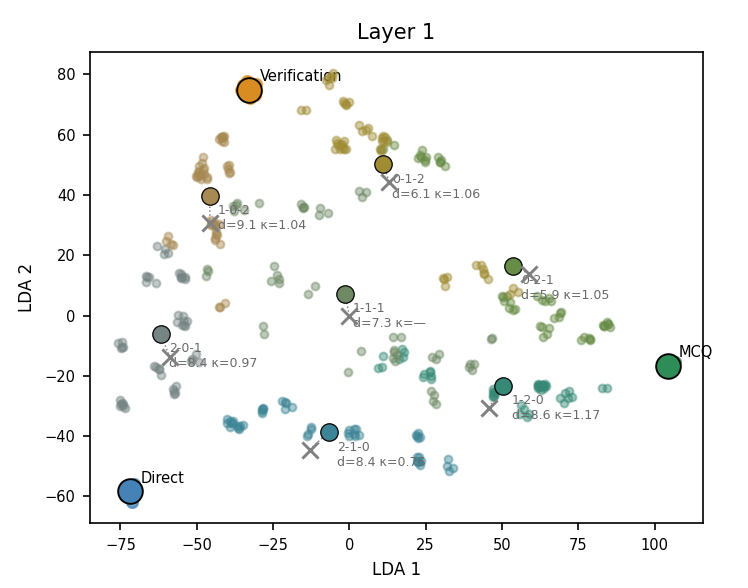
\includegraphics[width=0.95\linewidth]{arithmetic_layer_sweep_projections_Llama-3B_layer1.png}
    \end{subfigure}
    \hfill
    \begin{subfigure}{0.30\textwidth}
        \centering
        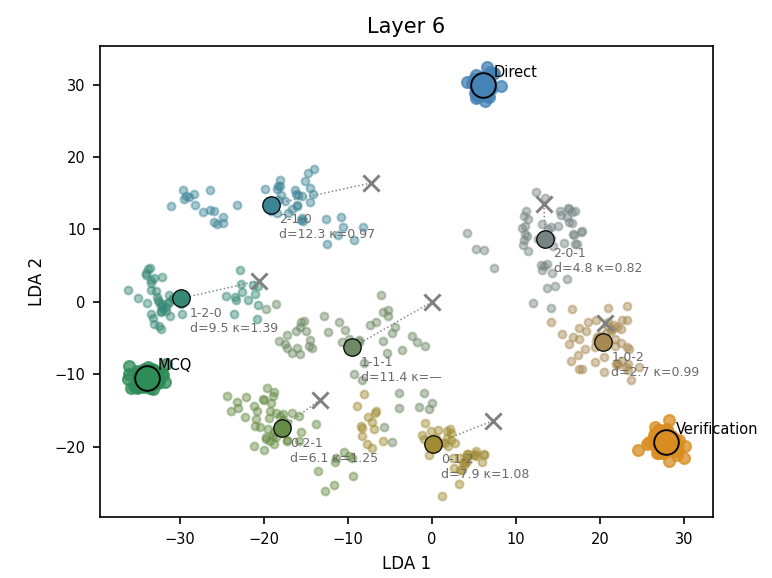
\includegraphics[width=0.95\linewidth]{arithmetic_layer_sweep_projections_Llama-3B_layer6.png}
    \end{subfigure}
    \hfill
    \begin{subfigure}{0.30\textwidth}
        \centering
        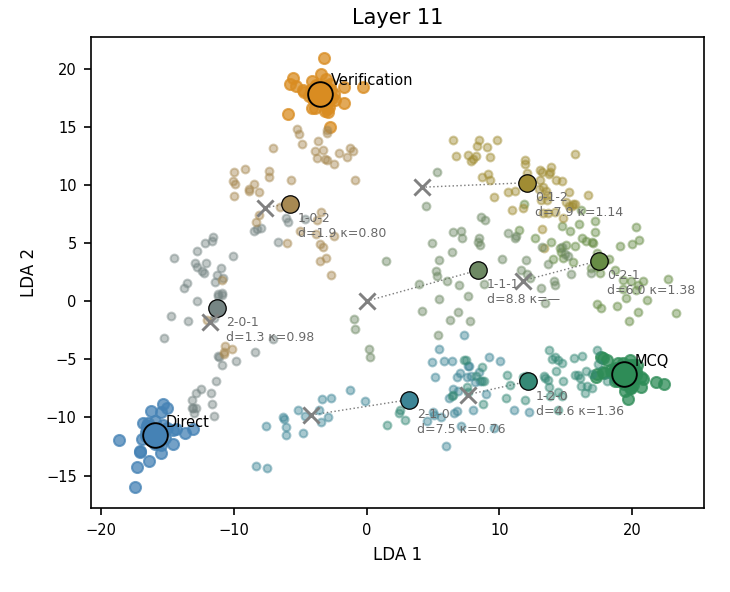
\includegraphics[width=0.95\linewidth]{arithmetic_layer_sweep_projections_Llama-3B_layer11.png}
    \end{subfigure}

    \begin{subfigure}{0.30\textwidth}
        \centering
        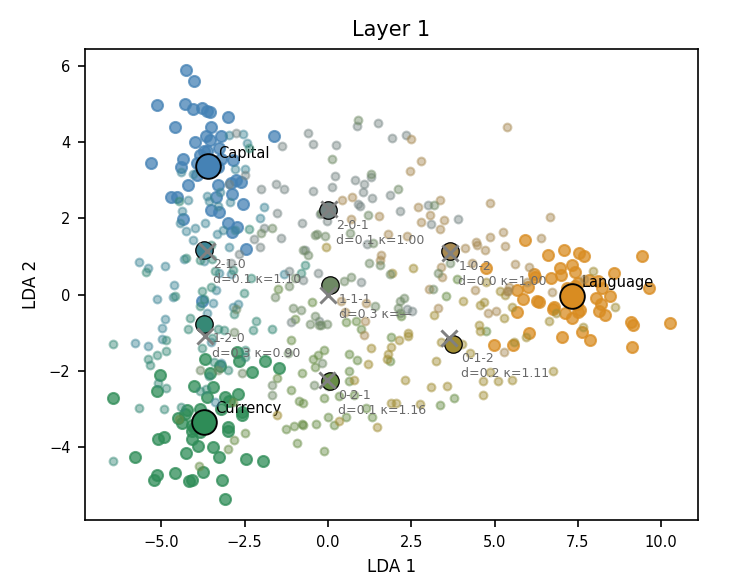
\includegraphics[width=0.95\linewidth]{entity_layer_sweep_projections_Llama-3B_layer1.png}
    \end{subfigure}
    \hfill
    \begin{subfigure}{0.30\textwidth}
        \centering
        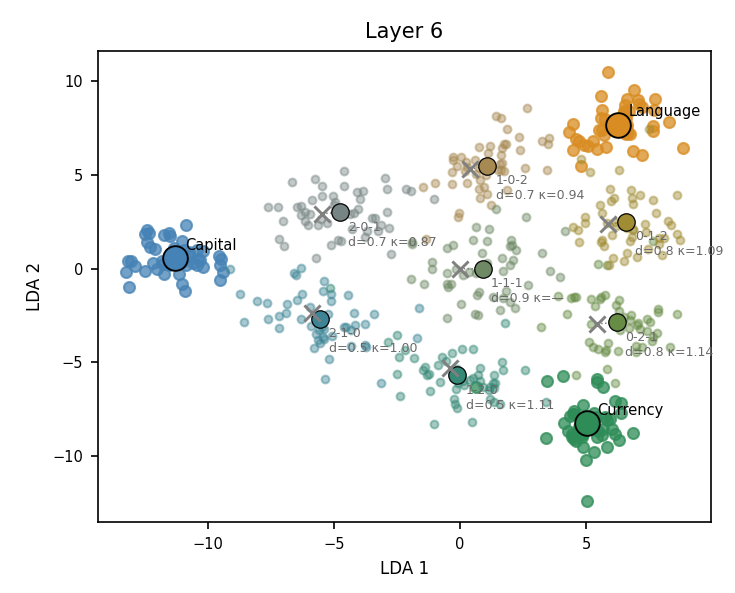
\includegraphics[width=0.95\linewidth]{entity_layer_sweep_projections_Llama-3B_layer6.png}
    \end{subfigure}
    \hfill
    \begin{subfigure}{0.30\textwidth}
        \centering
        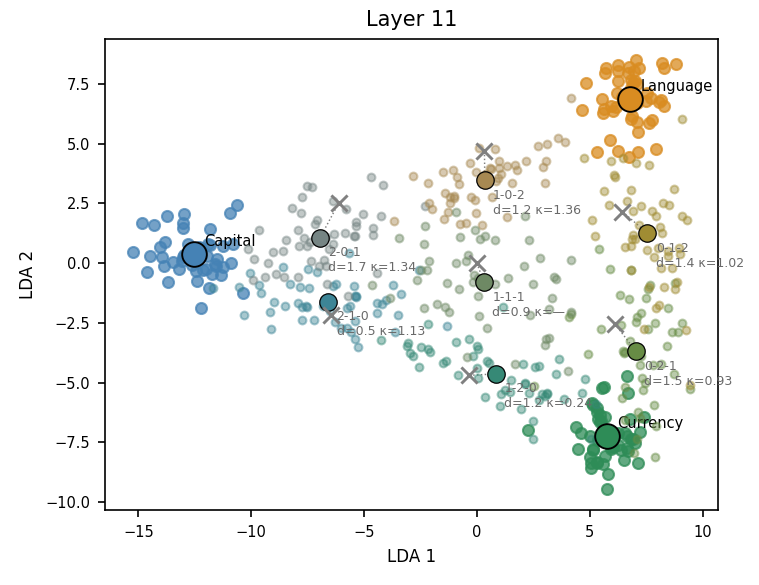
\includegraphics[width=0.95\linewidth]{entity_layer_sweep_projections_Llama-3B_layer11.png}
    \end{subfigure}
    
    \begin{subfigure}{0.30\textwidth}
        \centering
        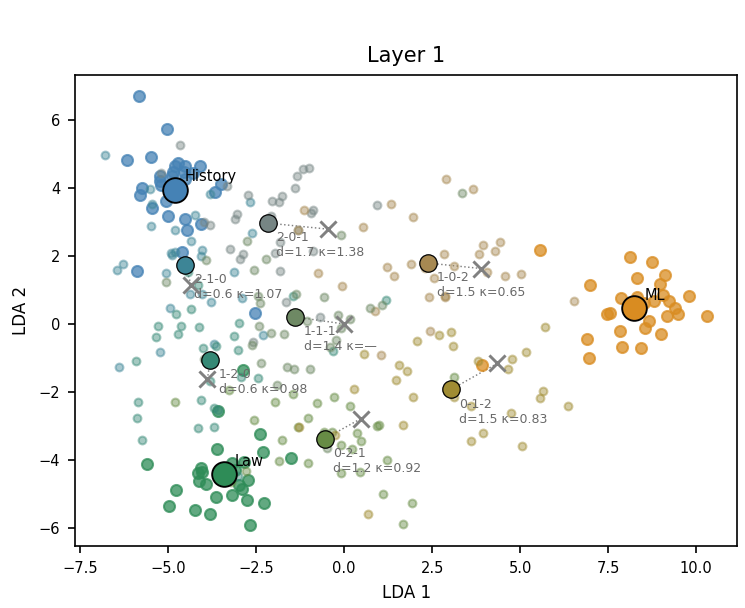
\includegraphics[width=0.95\linewidth]{mmlu_layer_sweep_projections_Llama-3B_layer1.png}
    \end{subfigure}
    \hfill
    \begin{subfigure}{0.30\textwidth}
        \centering
        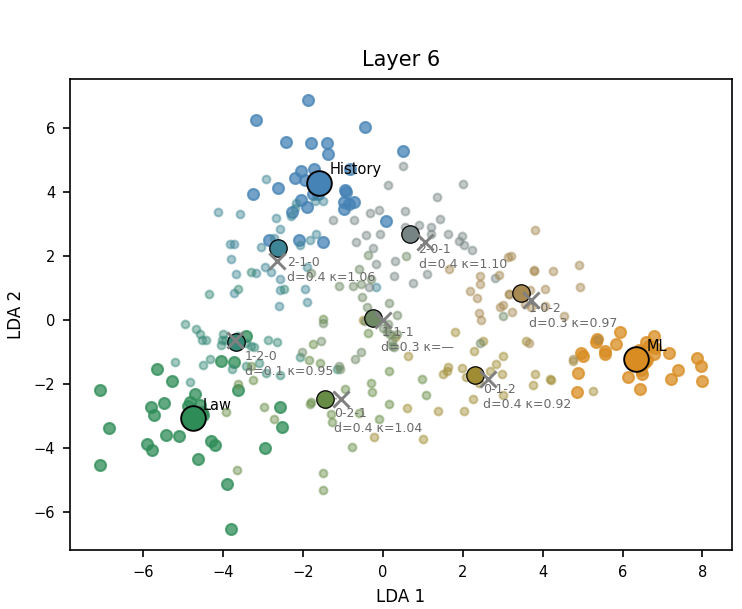
\includegraphics[width=0.95\linewidth]{mmlu_layer_sweep_projections_Llama-3B_layer6.png}
    \end{subfigure}
    \hfill
    \begin{subfigure}{0.30\textwidth}
        \centering
        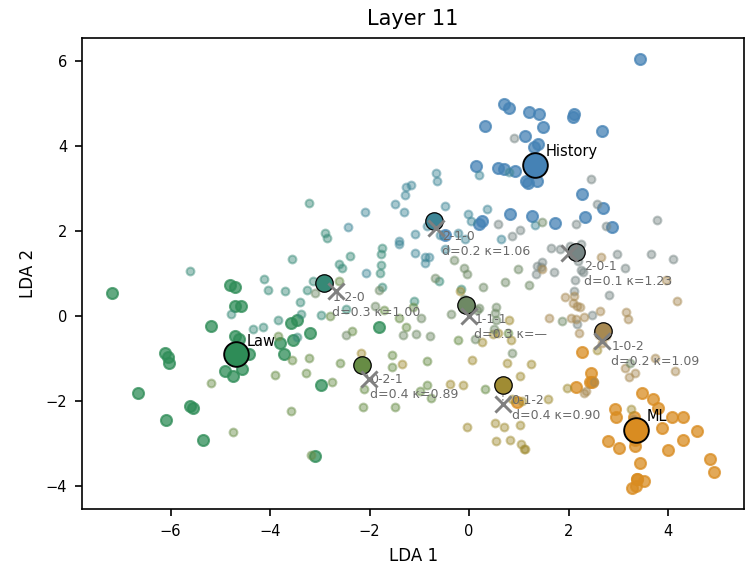
\includegraphics[width=0.95\linewidth]{mmlu_layer_sweep_projections_Llama-3B_layer11.png}
    \end{subfigure}
    \caption{Arithmetic (top), Entity (middle), and MMLU (bottom) task group contrast vector projections at layers 1, 6, and 11 for Llama 3.2 3B. \textbf{Colors:} Blue = Direct/Capital/History, Green = MCQ/Currency/ML, Orange = Verification/Language/Law respectively. \textbf{Markers:} $\boldsymbol{\times}$~predicted centroid, $\bullet$~actual centroid for a ratio.}
    \label{fig:lda_projections}
\end{figure*}
\begin{figure*}[!t]
    \centering
    \begin{subfigure}{0.30\textwidth}
        \centering
        
\includegraphics[width=0.95\linewidth]{arithmetic_kappa_comparison_across_models.png}
        \caption{Arithmetic task group}
        \label{fig:arith_kappa}
    \end{subfigure}
    \hfill
    \begin{subfigure}{0.30\textwidth}
        \centering
        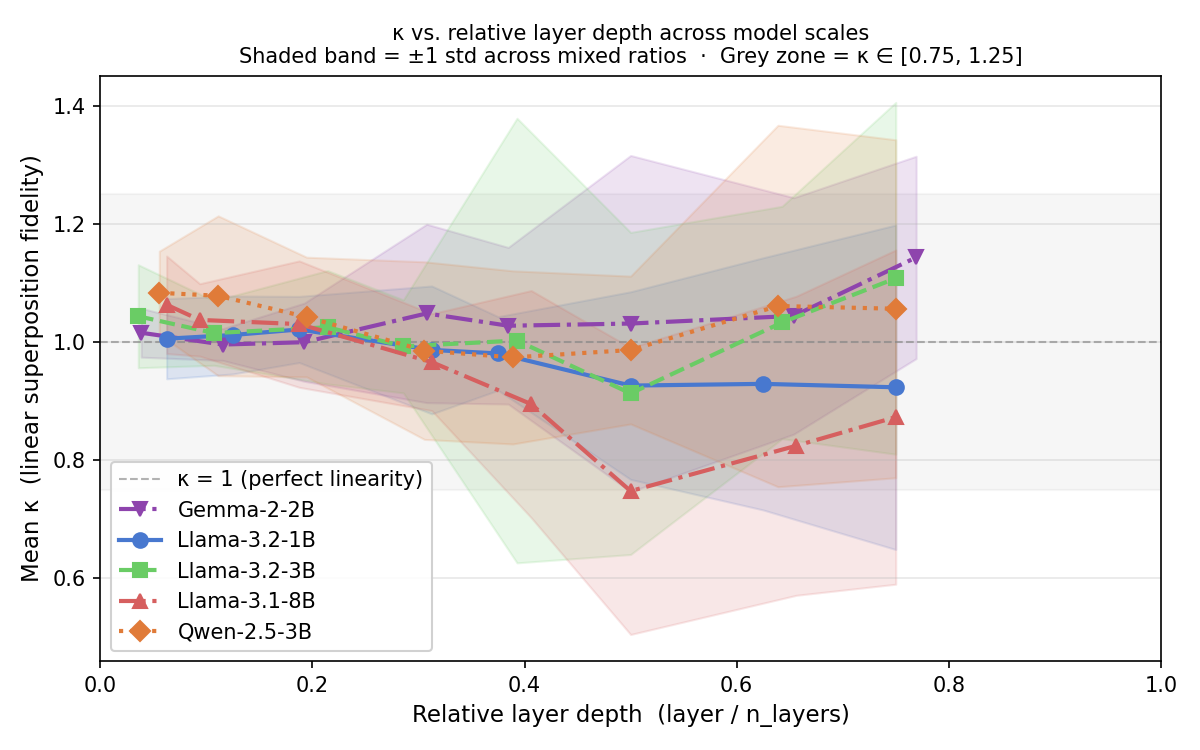
\includegraphics[width=0.95\linewidth]{entity_kappa_comparison_across_models.png}
        \caption{Entity task group}
        \label{fig:entity_kappa}
    \end{subfigure}
    \hfill
    \begin{subfigure}{0.30\textwidth}
        \centering
        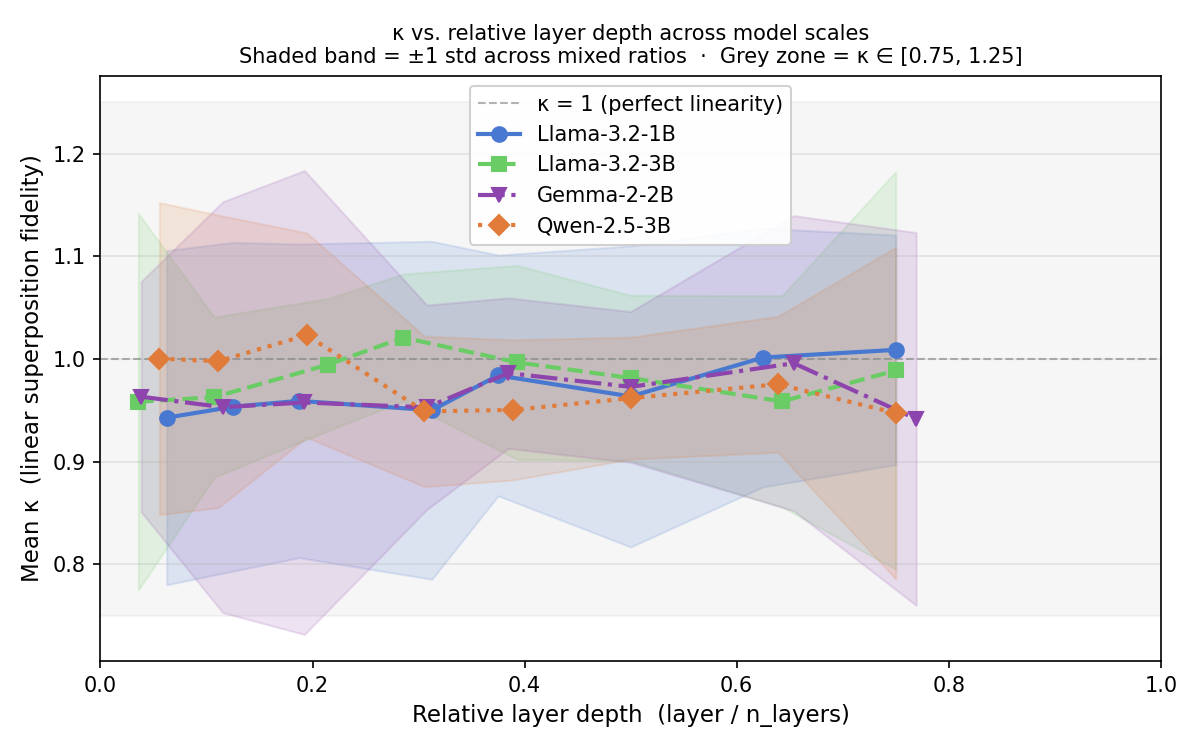
\includegraphics[width=0.95\linewidth]{mmlu_kappa_comparison_across_models.png}
        \caption{MMLU task group}
        \label{fig:mmlu_kappa}
    \end{subfigure}
    \caption{Cross model \(\kappa\) comparisons for (a) Arithmetic, (b) Entity, and (c) MMLU task groups for relative layer depths}
    \label{fig:cross_model_kappa}
\end{figure*}

\section{Empirical Verification of Linear Task Superposition}
This section tests the linear task superposition hypothesis at the representational level. We first examine the geometry of mixed-task contrast vectors, then evaluate whether mixture coefficients can be recovered from pure-task centroids, and finally discuss the empirical pattern across task groups and model families.

\subsection{Geometry of mixed-task representations}
In this section, we empirically collect and analyze contrast vectors with different in-context example ratios across the Arithmetic, Entity and MMLU task groups. We test this across different model families and sizes: Llama 3.2 1B, Llama 3.2 3B, Llama 3.1 8B \citep{grattafiori2024llama3}, Gemma 2 2B \citep{gemmateam2024gemma2}, and Qwen 2.5 3B \citep{yang2024qwen25}. We evaluate the instruction-tuned variants of these models to assess whether linear task vector superposition persists following instruction finetuning, extending prior work by \citet{xiong2024everything}, which established task superposition in pre-trained models, to practically deployed settings. Implementation details for prompt construction, layer selection, contrast vector extraction, and \(\kappa\) calculation are provided in \autoref{appendix:empirical_impl}. \\[1em]
Contrast vectors for the Llama 3.2 3B Instruct model projected onto a 2D LDA space are shown in \autoref{fig:lda_projections} for the Arithmetic, Entity, and MMLU task groups. Specifically, layers 1, 6, and 11 are chosen. Contrast vector projections for all the previously mentioned layer depths across all models and task groups are provided in \autoref{appendix:layer_sweep}. \\[1em]
Firstly, we observe a clear visual separation of pure task contrast vectors in the LDA space. Further, the mixed ratio contrast vector projections lie in between the pure task centroids along the directions predicted by a convex combination. Both of these visual observations are consistent with findings by \citet{xiong2024everything}. We further observe a clean visual clustering amongst contrast vector projections within each in-context ratio.
Additionally, in \autoref{fig:cross_model_kappa} we plot \(\kappa\) for each task group and model as a function of the relative layer depth, comparing it to the baseline \(\kappa = 1\) and against the range [0.75, 1.25]. Interestingly, the format-heavy Arithmetic task group shows the largest increase in \(\kappa\) variance with depth (0.25, vs 0.19 Entity, 0.024 MMLU), giving it the highest variance at deep layers. \\[1em]

\subsection{Recovering mixture coefficients}
\label{subsec:ols_formulation}
We next explore how this linearity hypothesis can be exploited to reconstruct the mixing coefficients of contrast vectors in a mixed task ICL prompt from the contrast vectors extracted from single task ICL prompts. We recover the coefficients with reparameterized OLS under the constraint that the coefficients sum to 1; the closed form solution is provided in \autoref{appendix:ols_sol}. \\[1em]
The OLS results are summarized by the per-ratio L2 errors in \autoref{fig:ols_l2}. Full recovered coefficients, 95\% bootstrap confidence intervals, and L2 errors are provided in \autoref{appendix:ols_results}.
\begin{figure}[th]
    \centering
    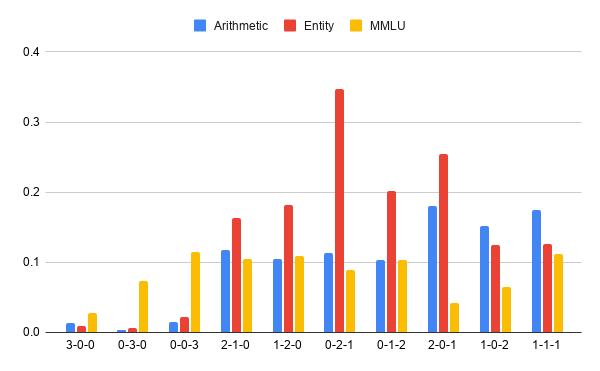
\includegraphics[width=\linewidth]{ols_l2_error_chart.png}
    \caption{Per ratio L2 errors across task groups}
    \label{fig:ols_l2}
\end{figure}

\subsection{Discussion}
In conclusion, we observe that \(\kappa\) remains close to 1 across all task groups and all model families and sizes specified, with a greater consistency in semantic-varying tasks than format-varying tasks. This provides evidence that task vectors do superpose linearly at a representational level, and this generalizes across the model families examined.

\section{Causal Validation through Contrast Vector Injection}
\subsection{Intervention methodology}

\subsection{Injection results}

\subsection{Implications}

\section{Limitations}

\section{Conclusion}
\clearpage
\bibliography{references}

\newpage
\onecolumn
\appendix

\section{Implementation details for empirical verification}
\label{appendix:empirical_impl}

\subsection*{Prompt construction}
For each of the 10 ratios listed in \ref{subsec:icl_ratios}, \(n\) samples of in-context examples and test questions are created for each task group. \(n = 50\) for the Arithmetic and Entity task groups and \(n = 30\) for MMLU tasks. \\[1em]
For arithmetic tasks, \texttt{op1} and \texttt{op2} are sampled from the range [1, 49] and are formatted as Direct, MCQ, or Verification tasks. For entity tasks, countries are sampled and their corresponding entities are extracted based on the ratio. For MMLU tasks, questions for a sample are extracted from each task (subject/domain) based on the ratio. \\[1em]
For a given task group and ratio, each sample constitutes (1) the in context examples concatenated with the test question to produce the few shot prompt, and (2) the corresponding test question, used as the zero-shot baseline. For all three task groups, the test question is extracted from a heldout pool disjoint from the in-context examples. Implementation details on sampling the ICL examples and test question can be found in \autoref{appendix:sampling}.

\subsection*{Layer selection}
We use the following relative layer depths for each model: [0.05, 0.1, 0.2, 0.3, 0.4, 0.5, 0.65, 0.75]. The higher density in earlier layers is intended to capture the region where task-relevant information is most concentrated, motivated by findings that task and function vectors are most effective when injected in the early-to-middle layers of autoregressive LLMs \citep{Hendel2023-yk, todd2023function}.

\subsection*{Contrast vector extraction}
For each sample, we first collect the activations at the final token of the residual stream at the assistant boundary turn. Since these activations are independent of the task ratio in in-context examples, they are precomputed and stored in a temporary cache for efficiency. This is done by rotating the task corresponding to the test question for each sample. That is, for sample index \texttt{i}, the test question is drawn from the task \texttt{TASKS[i \% num\_tasks]}. \\[1em]
Next, for each ratio, we conduct another forward pass to collect the activations at the assistant header when given the few shot prompts and the corresponding test questions used in the zero shot prompts. \\[1em]
The stored zero shot activations are then subtracted from the corresponding few shot activations to produce contrast vectors at each layer of the model for each ratio. For visualizing these vectors, following the method used by \citet{xiong2024everything}, we use LDA projection. LDA is fit on the pure condition contrast vectors only ((3, 0, 0), (0, 3, 0), and (0, 0, 3)). This is then used to transform the contrast vectors from all 10 ratios. A separate LDA is fit per layer per task group.

\subsection*{Calculating $\kappa$}
The above contrast vectors are then used to compute \(\mu_r^l, \hat{\mu_r}^l\), and \(\mu^l\) as described in \ref{subsec:kappa} for each layer at each ratio. The calculated values of \(\kappa\) are then stored per model and task group. \(\kappa\) is calculated using the original contrast vectors, not the LDA projected vectors, providing a measurement of linearity in the original activation space. \\[1em]
Further, as stated in \ref{subsec:kappa}, \(\kappa\) is not well defined for the 1-1-1 ratio and is therefore not computed. More details on avoiding computing \(\kappa\) in undefined cases can be found in \autoref{appendix:kappa_edge}.

\section{Implementation details for task group sampling}
\label{appendix:sampling}

\subsection*{Arithmetic}
First, a pool of 200 in-context and 50 test pairs \((\texttt{op1}, \texttt{op2})\), with each \(\texttt{op1, op2} \in [1 ,49]\), are generated using seeds 42 and 43 respectively. Duplicate pairs are re-generated until the ICL and test pools are disjoint. Thus, while the same \texttt{(op1, op2)} pair can appear in more than 1 in-context example, the in-context and test pools are disjoint. For each sample using ratio \(r\) of task combinations, 3 in-context \texttt{op} pairs and 1 test \texttt{op} pair are drawn without replacement. Each of the ICL pairs are formatted according to the ratio \(r\) and are concated with the test \texttt{op} pair. \\[1em]
\textbf{Generating distractors for multiple choice}- the distractors are within 10 of the true value of \(\texttt{op1 + op2}\). This is to prevent lexical differences in the options having an unintended influence on the intended task to represent. \\[1em]
For each ratio \(r\), we use \(n = 50\) samples.
\subsection*{Entity}
We manually curate a dataset of 96 countries and map each to its capital, currency, and language. This dataset is partitioned into an in-context pool of 66 countries and a test pool of 30 countries, making the two pools disjoint. 
To generate the in-context examples for a prompt, we sample countries without replacement from the in-context pool for each task according to the ratio \(r\). This guarantees that countries are not repeated for a single task (that is, \texttt{France -> Euro} does not appear twice in one sample prompt), but allows for cross-task duplication of countries (that is, \texttt{France -> Euro} and \texttt{France -> Paris} can appear in the same prompt). The test question is separately drawn from the test pool. \\[1em]
We use \(n = 50\) samples for each in-context ratio. We do not add an assistant trigger in the user prompt after the test question; the prompt format is consistent across tasks and ratios.
\subsection*{MMLU}
First, the questions from each subject (History, Law, ML) are shuffled by a seed (42). We use the test split of the MMLU dataset to avoid prior exposure of the train set questions to influence the model's behavior. Next, the questions for each subject are partitioned into pools of upto 150 in-context questions and 20 test questions. Since ML has 112 questions in the MMLU dataset, we save 20 questions for the test pool and use the remaining 92 questions as the in-context pool. This guarantees the in-context and test pools are disjoint. \\[1em]
For each ratio \(r\) of task combinations, \(n = 30\) samples are independently constructed, drawing 3 questions from the in-context pool according to \(r\) and one test set question. This is lower than the number of samples for the arithmetic and entity groups due to practical hardware constraints but is sufficient for statistically significant results.

\section{Handling undefined \(\kappa\) cases}
\label{appendix:kappa_edge}

\section{Layer sweep projection figures}
\label{appendix:layer_sweep}

\subsection*{Arithmetic}
\begin{figure}[H]
    \centering
    \begin{subfigure}{0.48\linewidth}
        \centering
        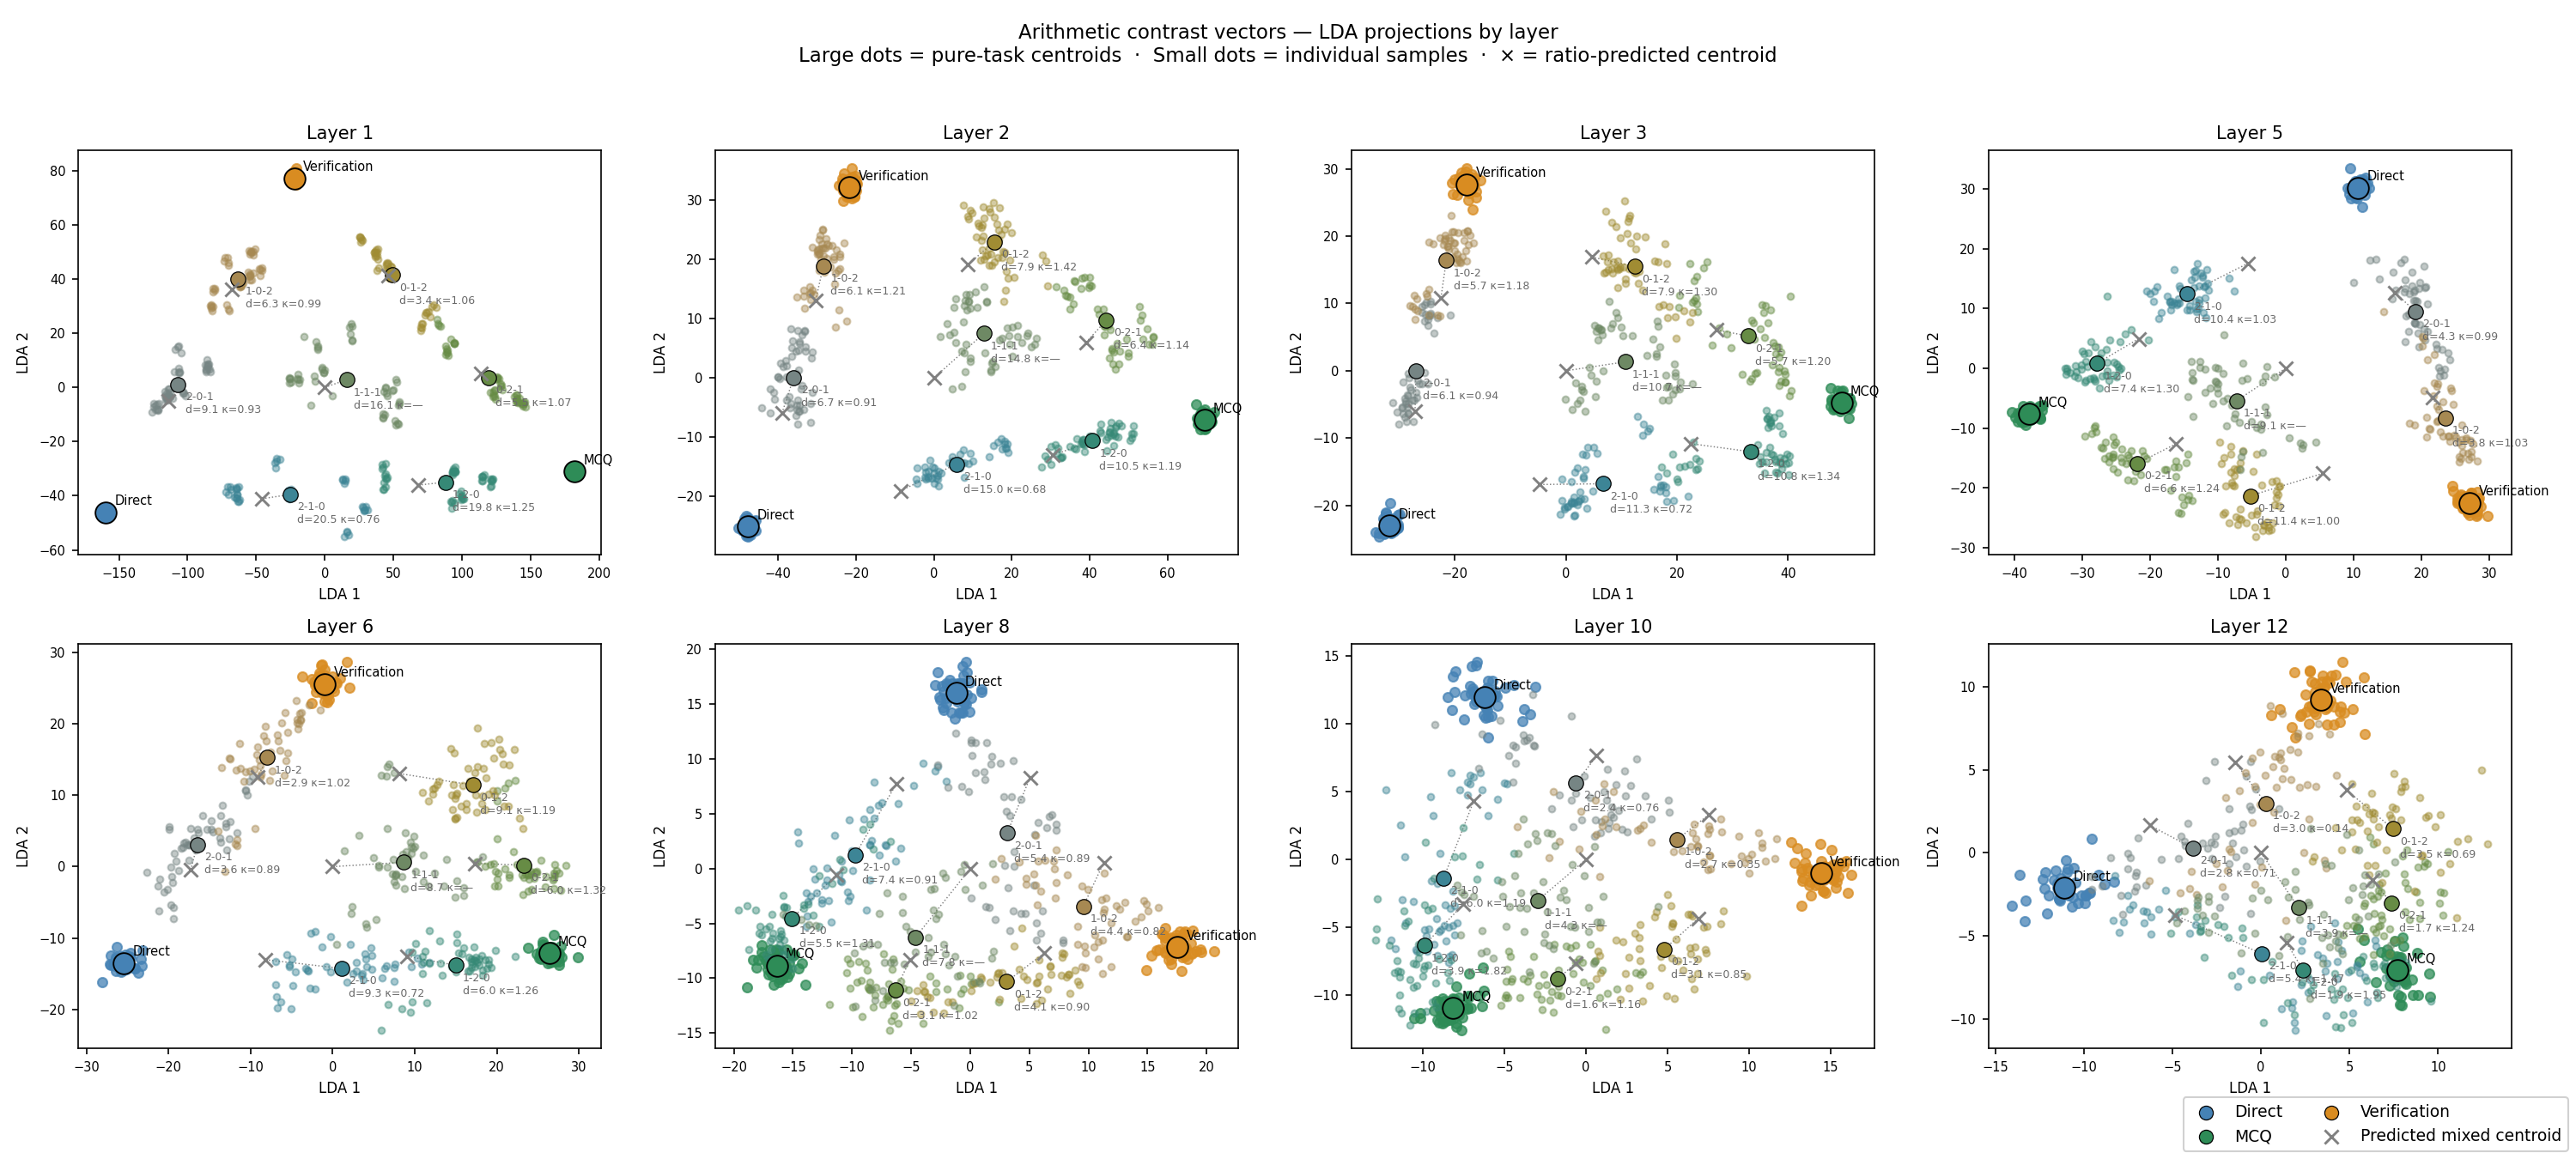
\includegraphics[width=\linewidth]{arithmetic_layer_sweep_projections_Llama-1B_rotated.png}
        \caption{Llama 3.2 1B}
    \end{subfigure}
    \hfill
    \begin{subfigure}{0.48\linewidth}
        \centering
        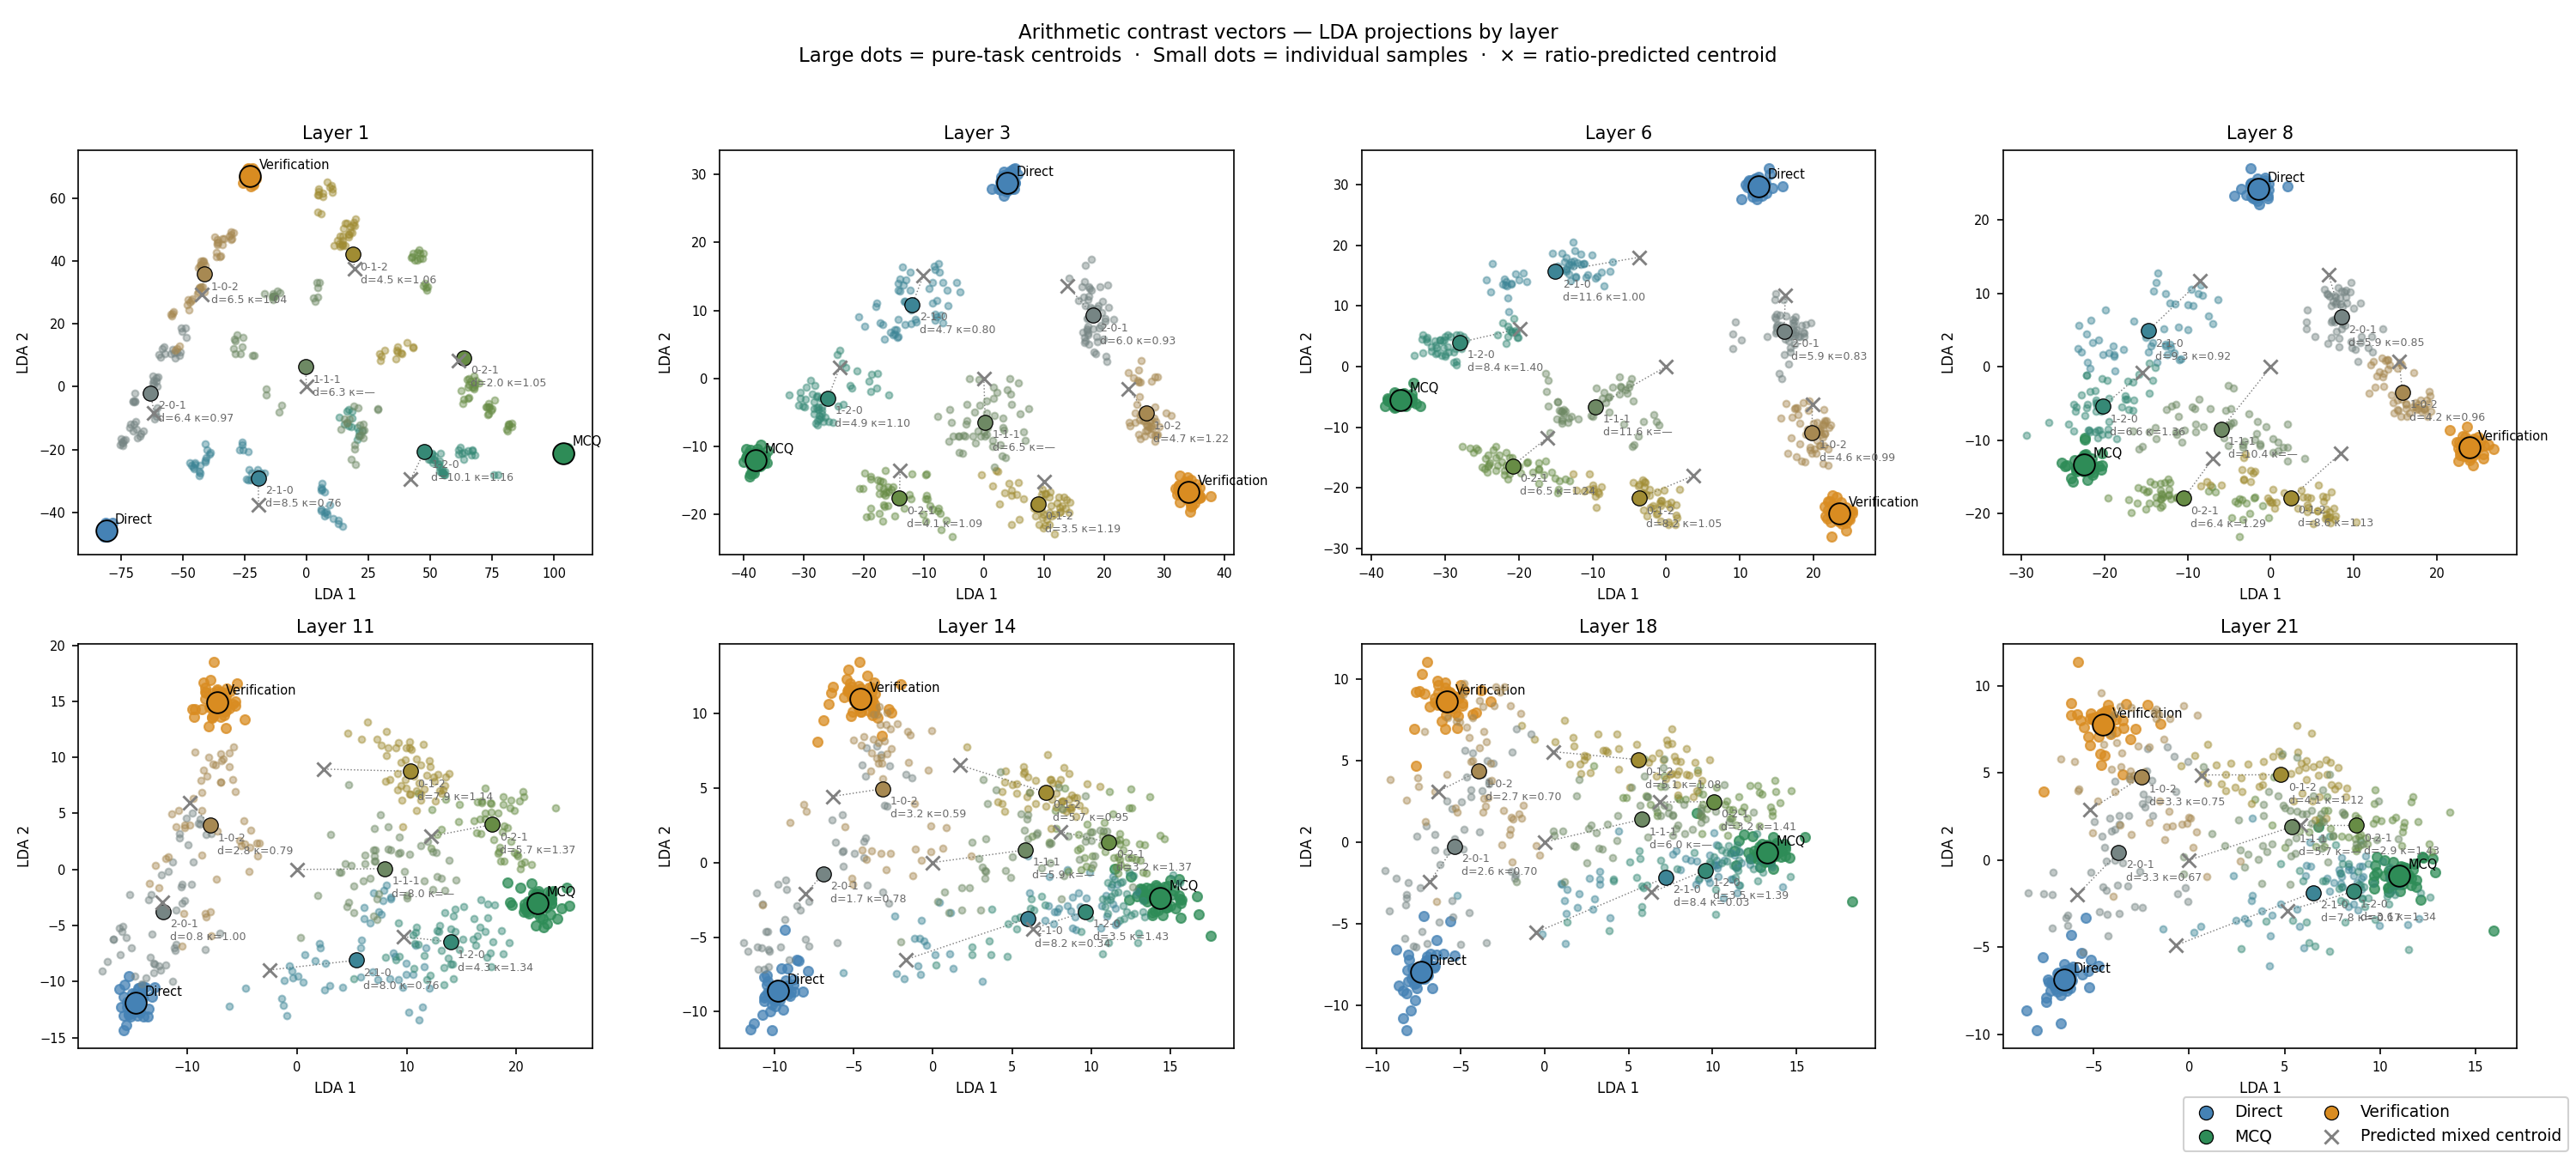
\includegraphics[width=\linewidth]{arithmetic_layer_sweep_projections_Llama-3B_rotated.png}
        \caption{Llama 3.2 3B}
    \end{subfigure}

    \begin{subfigure}{0.48\linewidth}
        \centering
        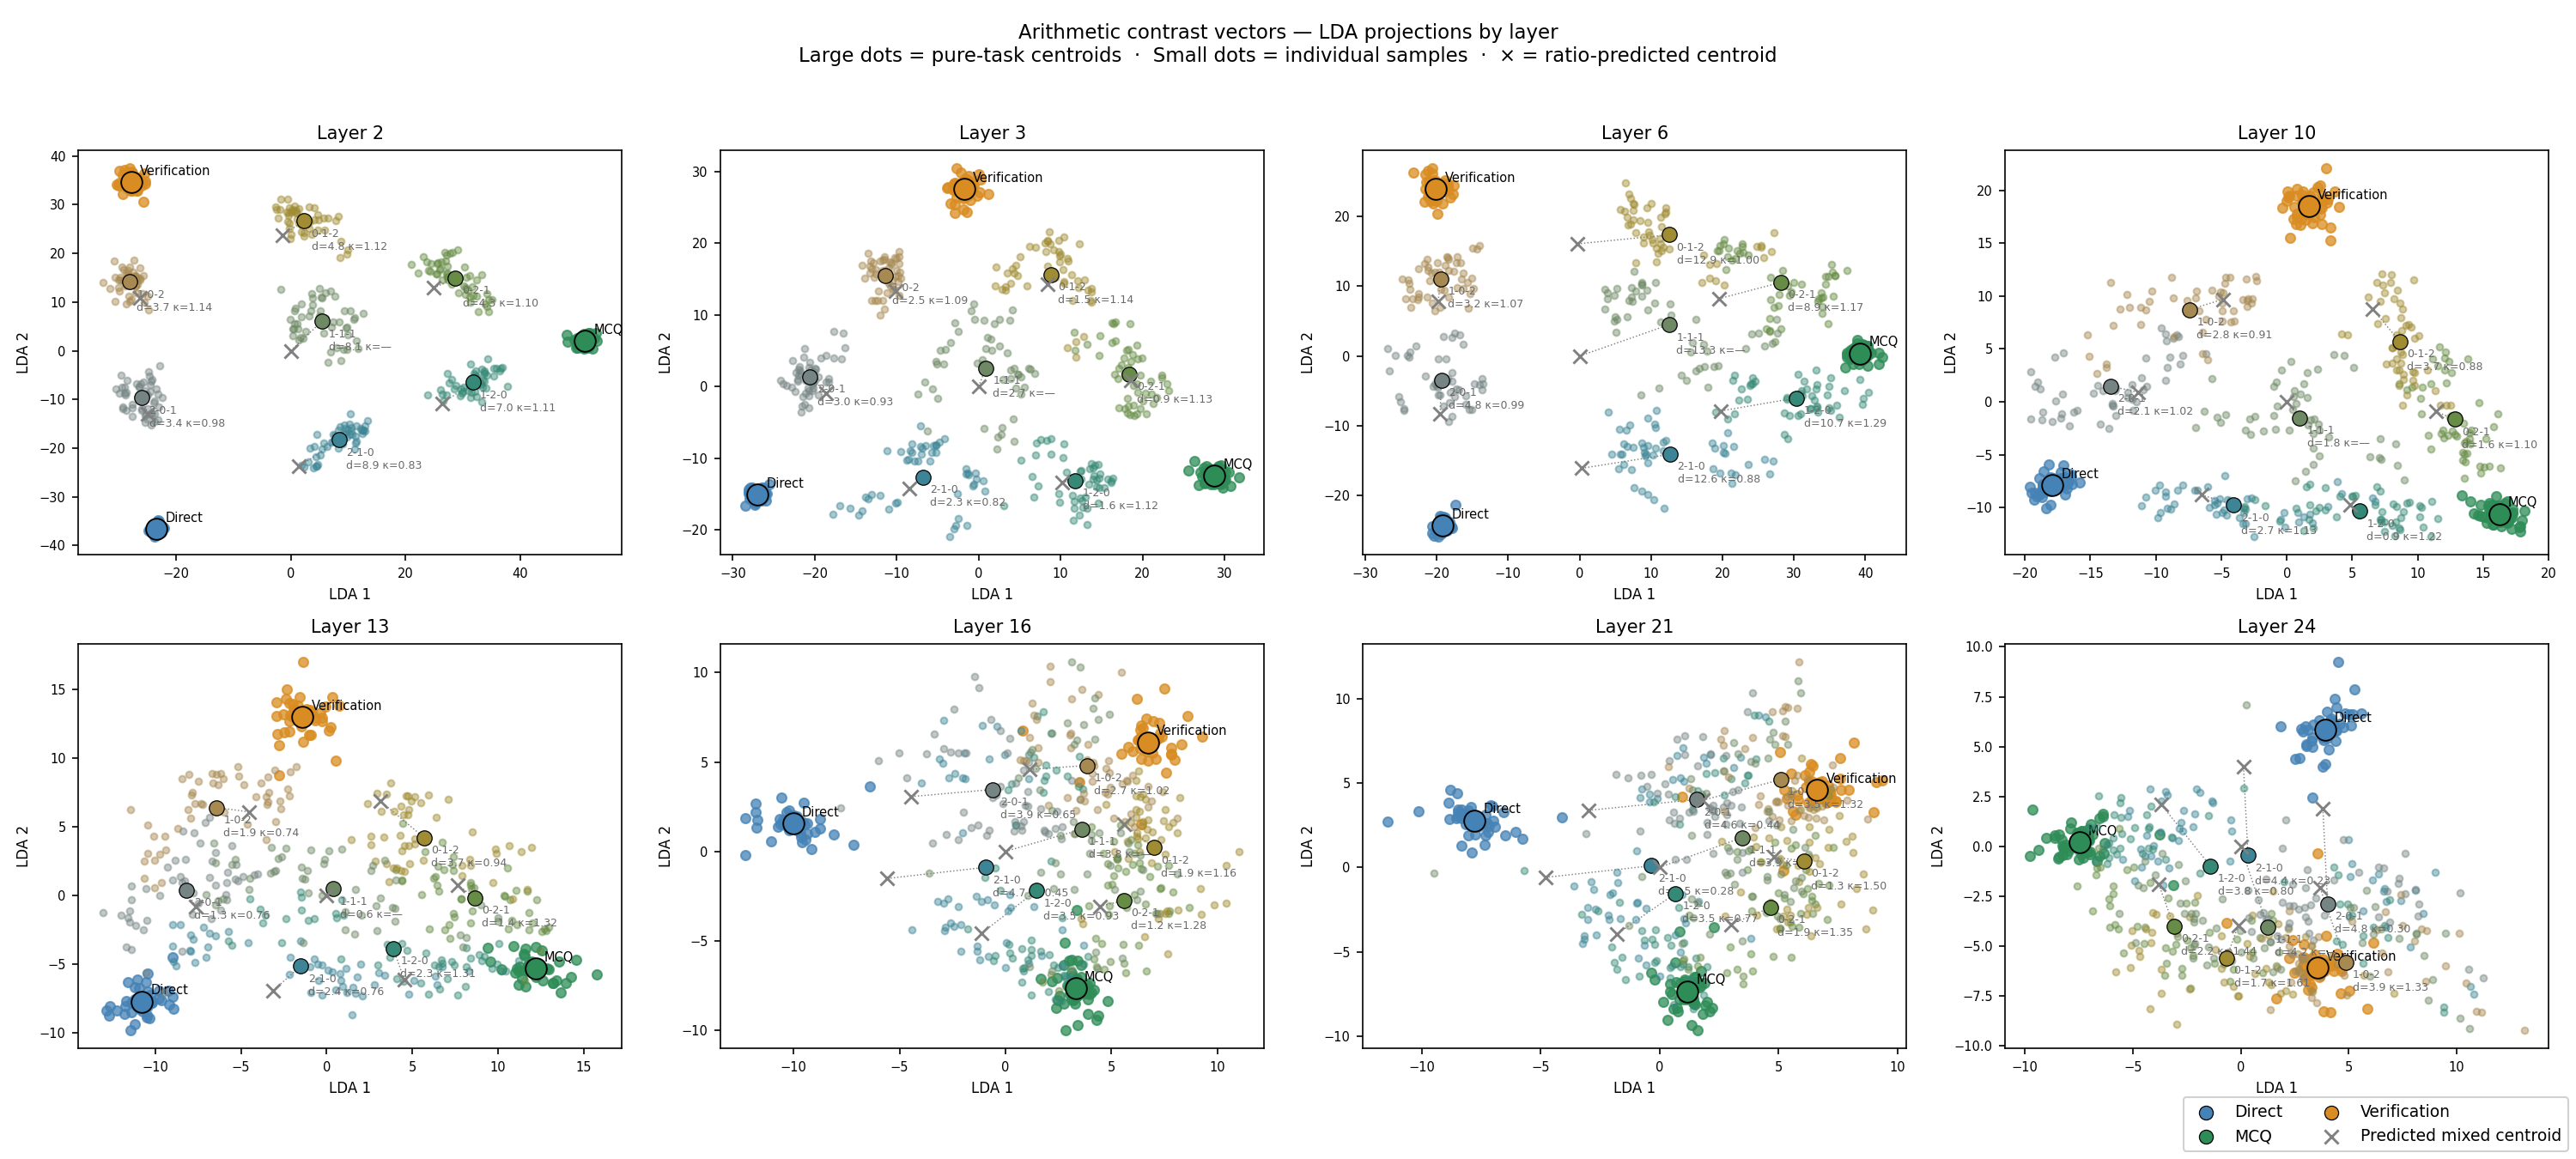
\includegraphics[width=\linewidth]{arithmetic_layer_sweep_projections_Llama-8B_rotated.png}
        \caption{Llama 3.1 8B}
    \end{subfigure}
    \hfill
    \begin{subfigure}{0.48\linewidth}
        \centering
        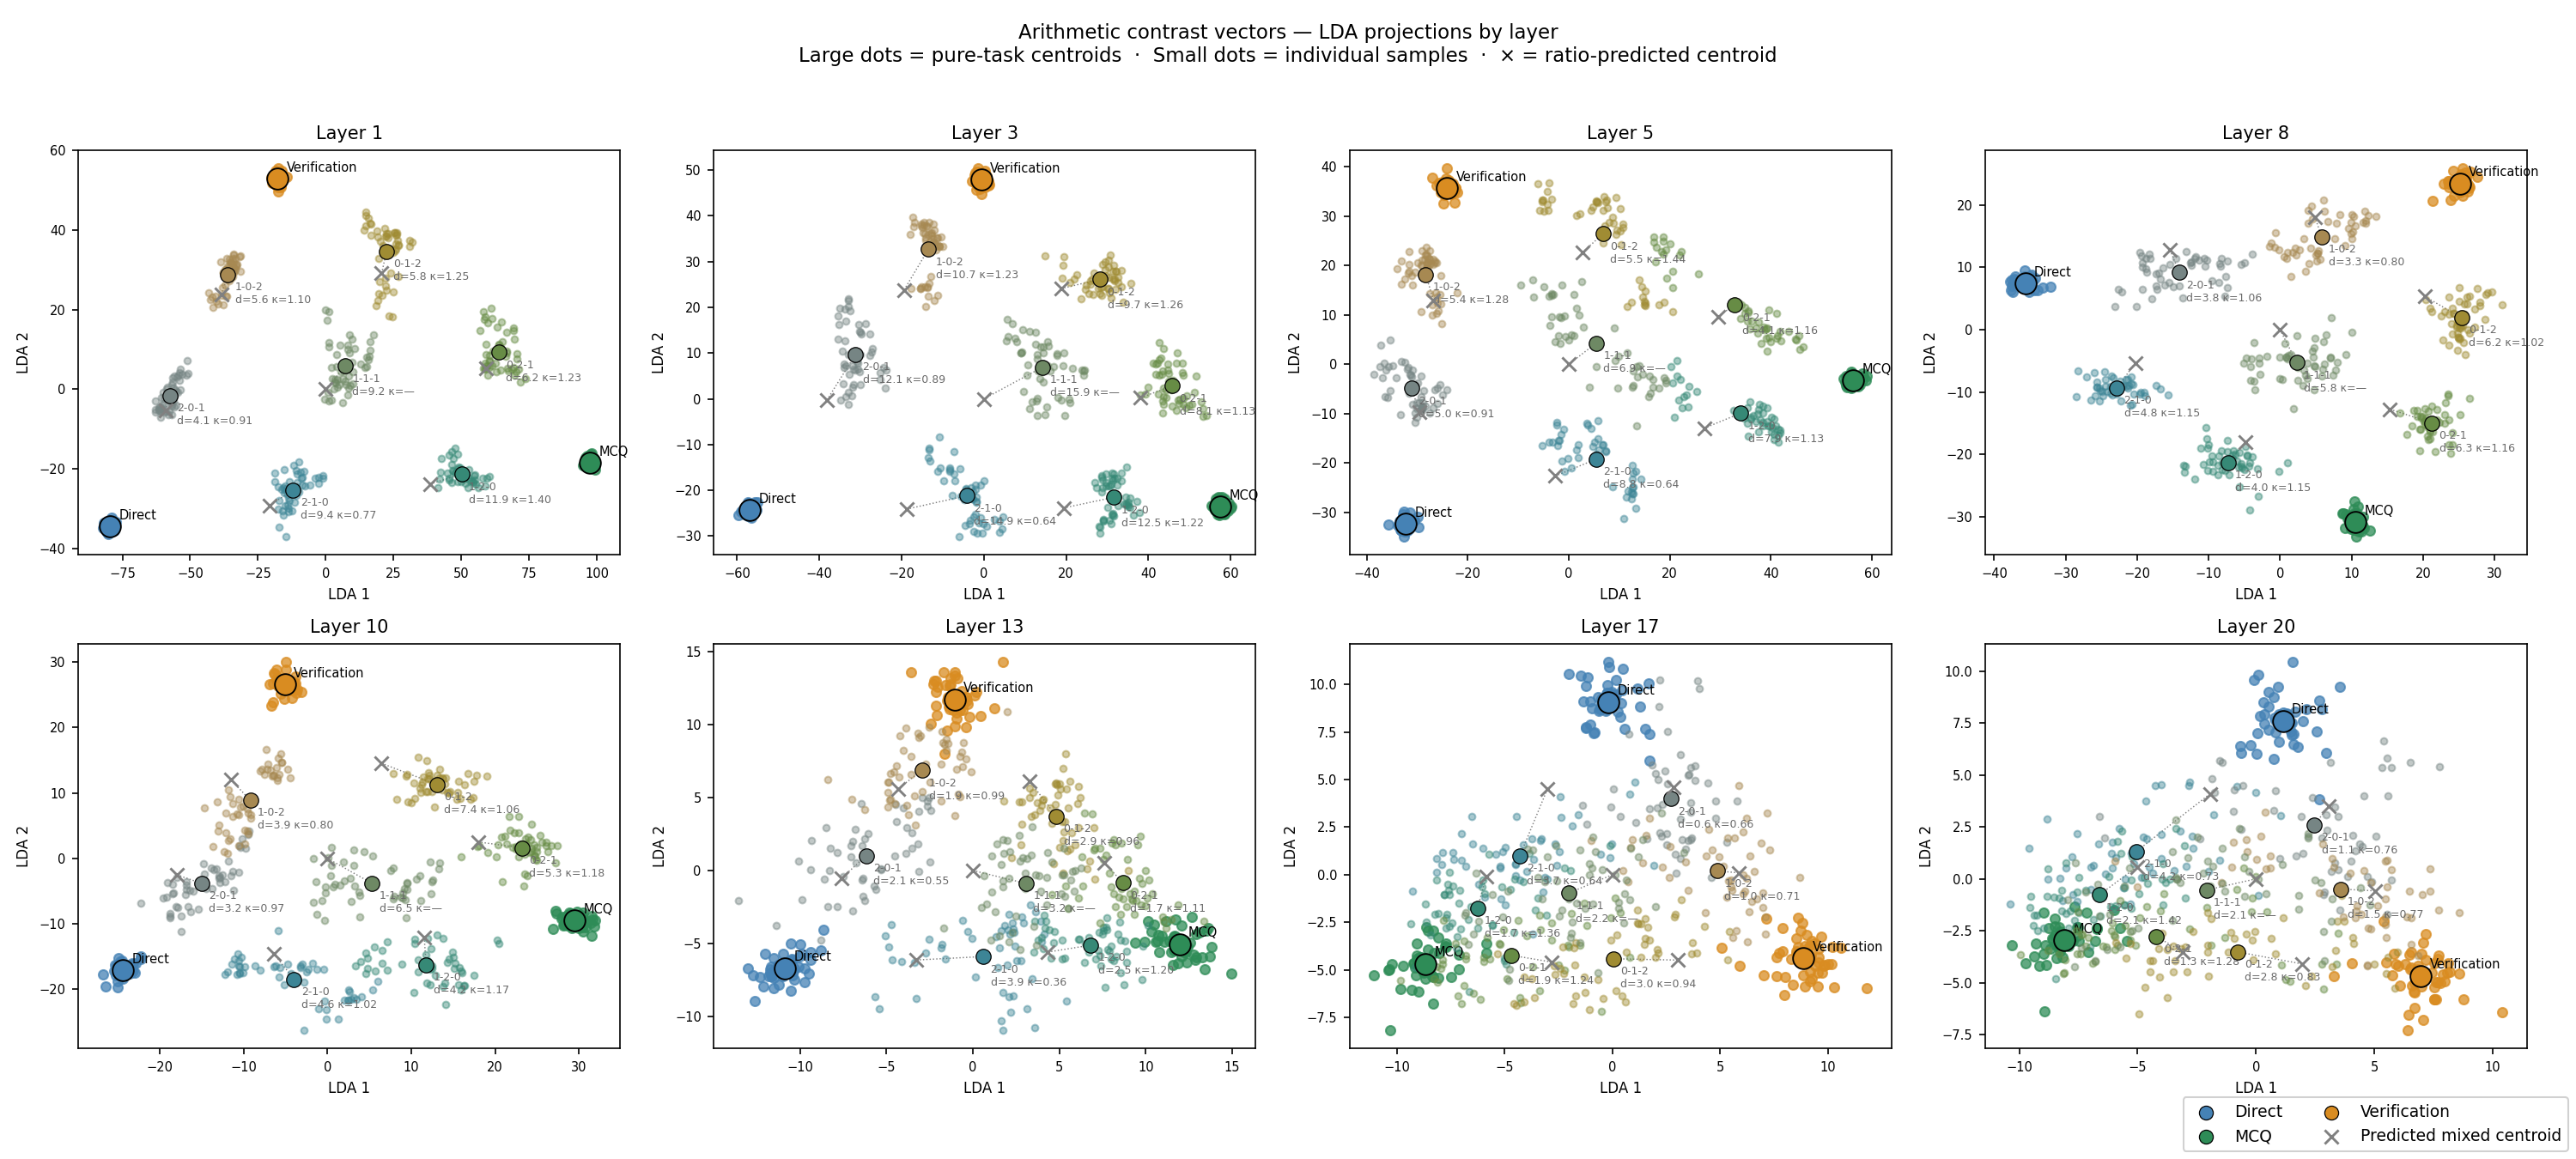
\includegraphics[width=\linewidth]{arithmetic_layer_sweep_projections_Gemma-2B_rotated.png}
        \caption{Gemma 2 2B}
    \end{subfigure}

    \begin{subfigure}{0.48\linewidth}
        \centering
        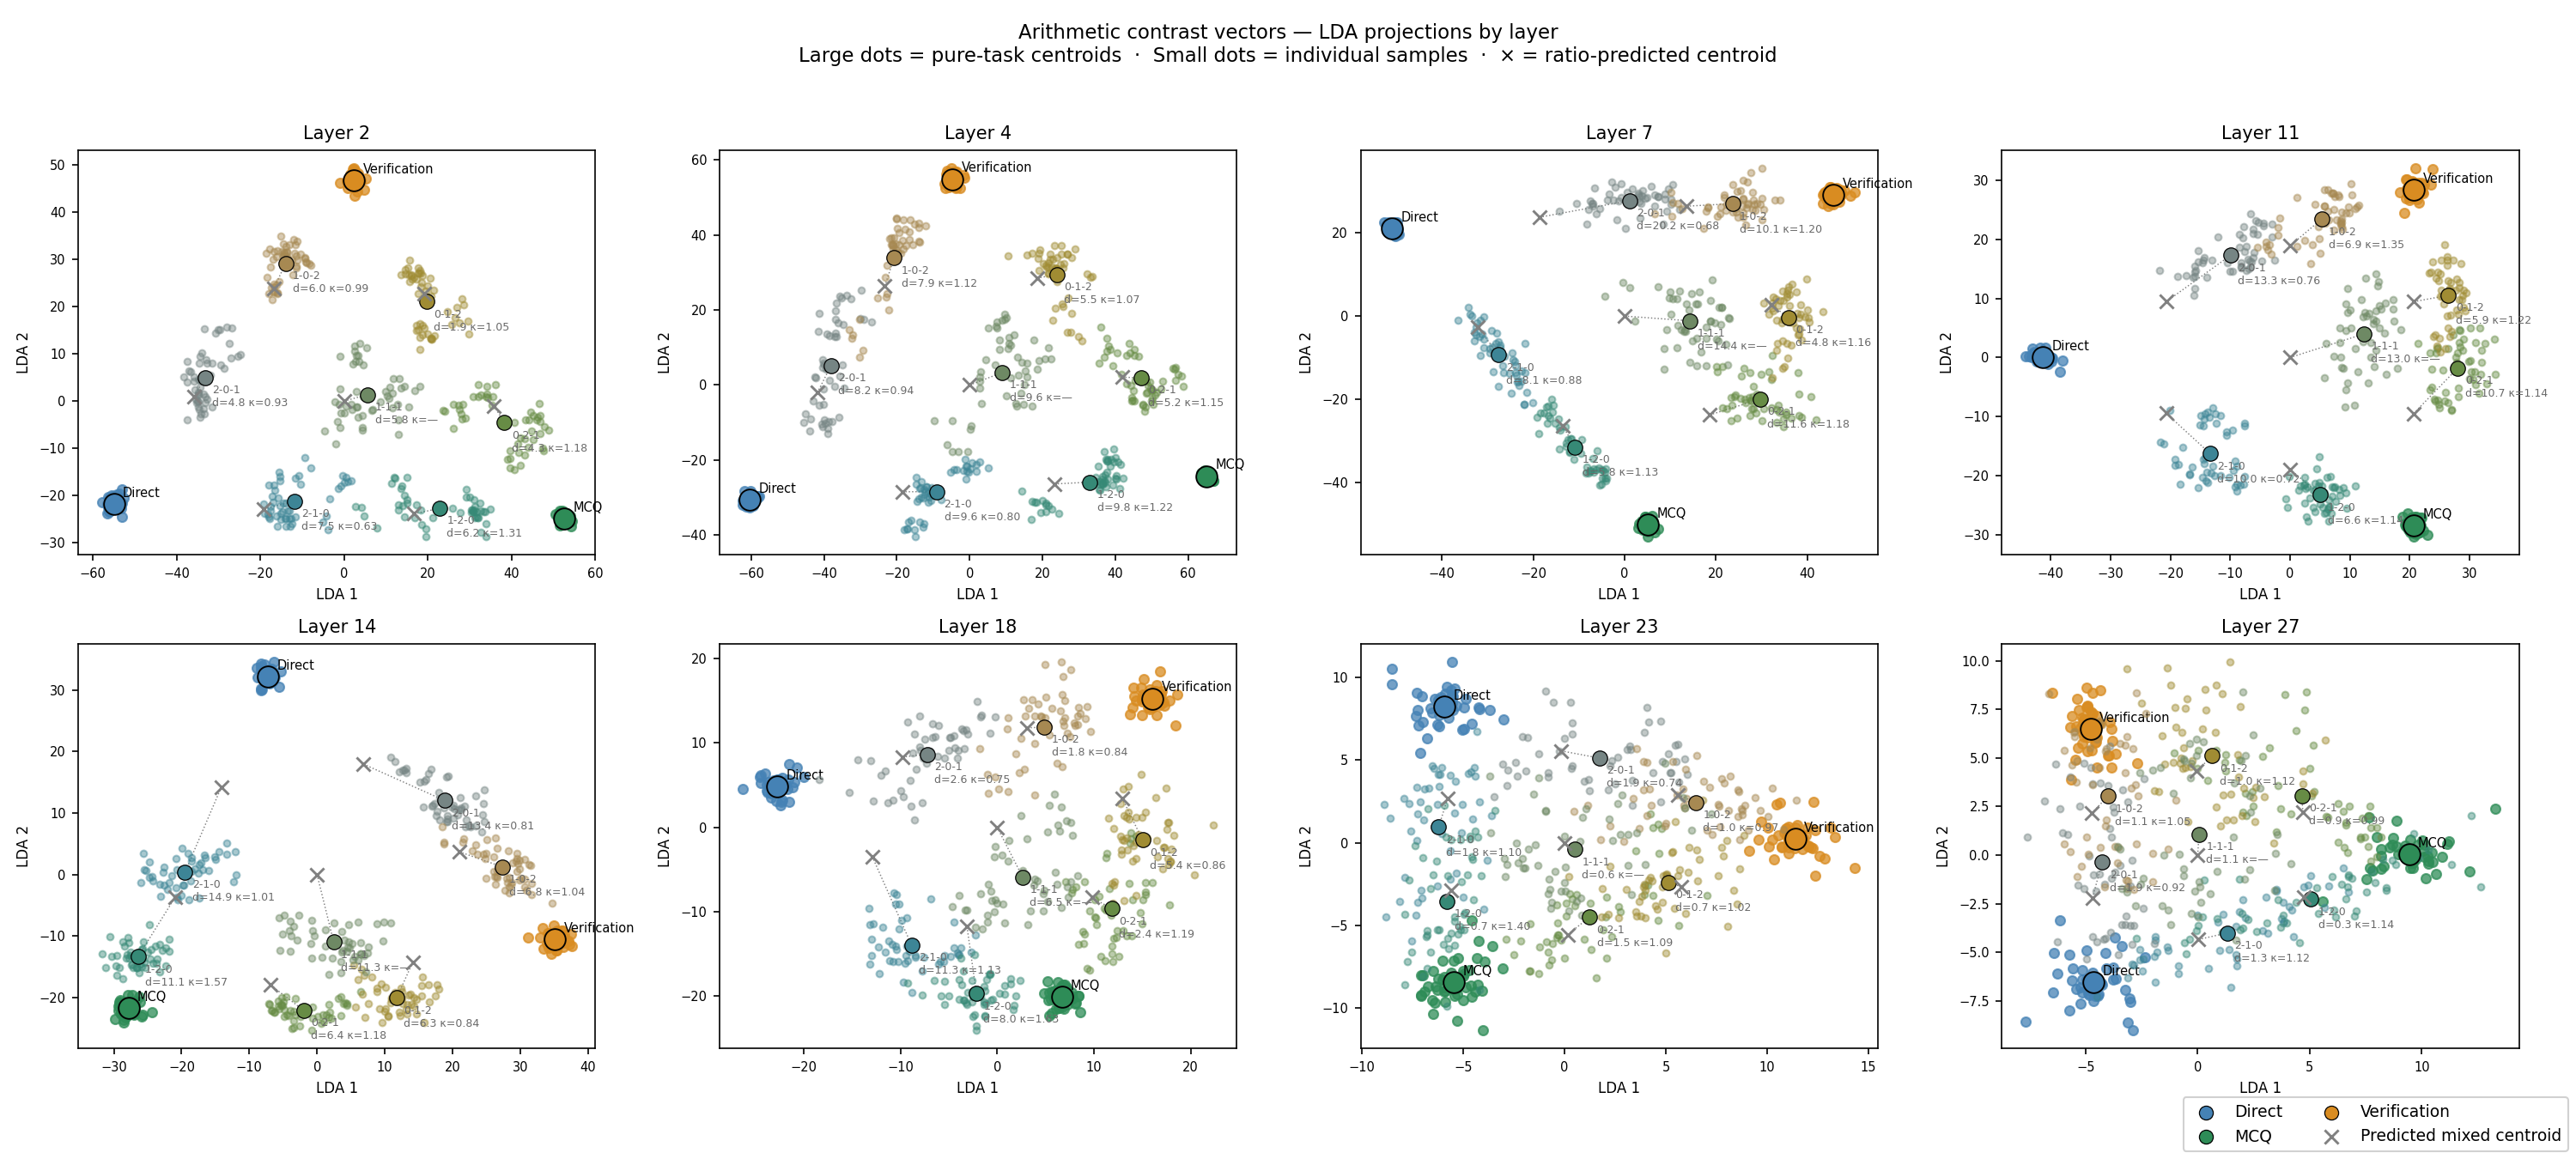
\includegraphics[width=\linewidth]{arithmetic_layer_sweep_projections_Qwen-3B_rotated.png}
        \caption{Qwen 2.5 3B}
    \end{subfigure}
    \caption{Arithmetic layer sweep projections across models. \textbf{Colors:} Blue = Direct, Green = MCQ, Orange = Verification. \textbf{Markers:} $\boldsymbol{\times}$~predicted centroid, $\bullet$~actual centroid for a ratio.}
    \label{fig:arith_results}
\end{figure}

\subsection*{MMLU}
\begin{figure}[H]
    \centering
    \begin{subfigure}{0.48\linewidth}
        \centering
        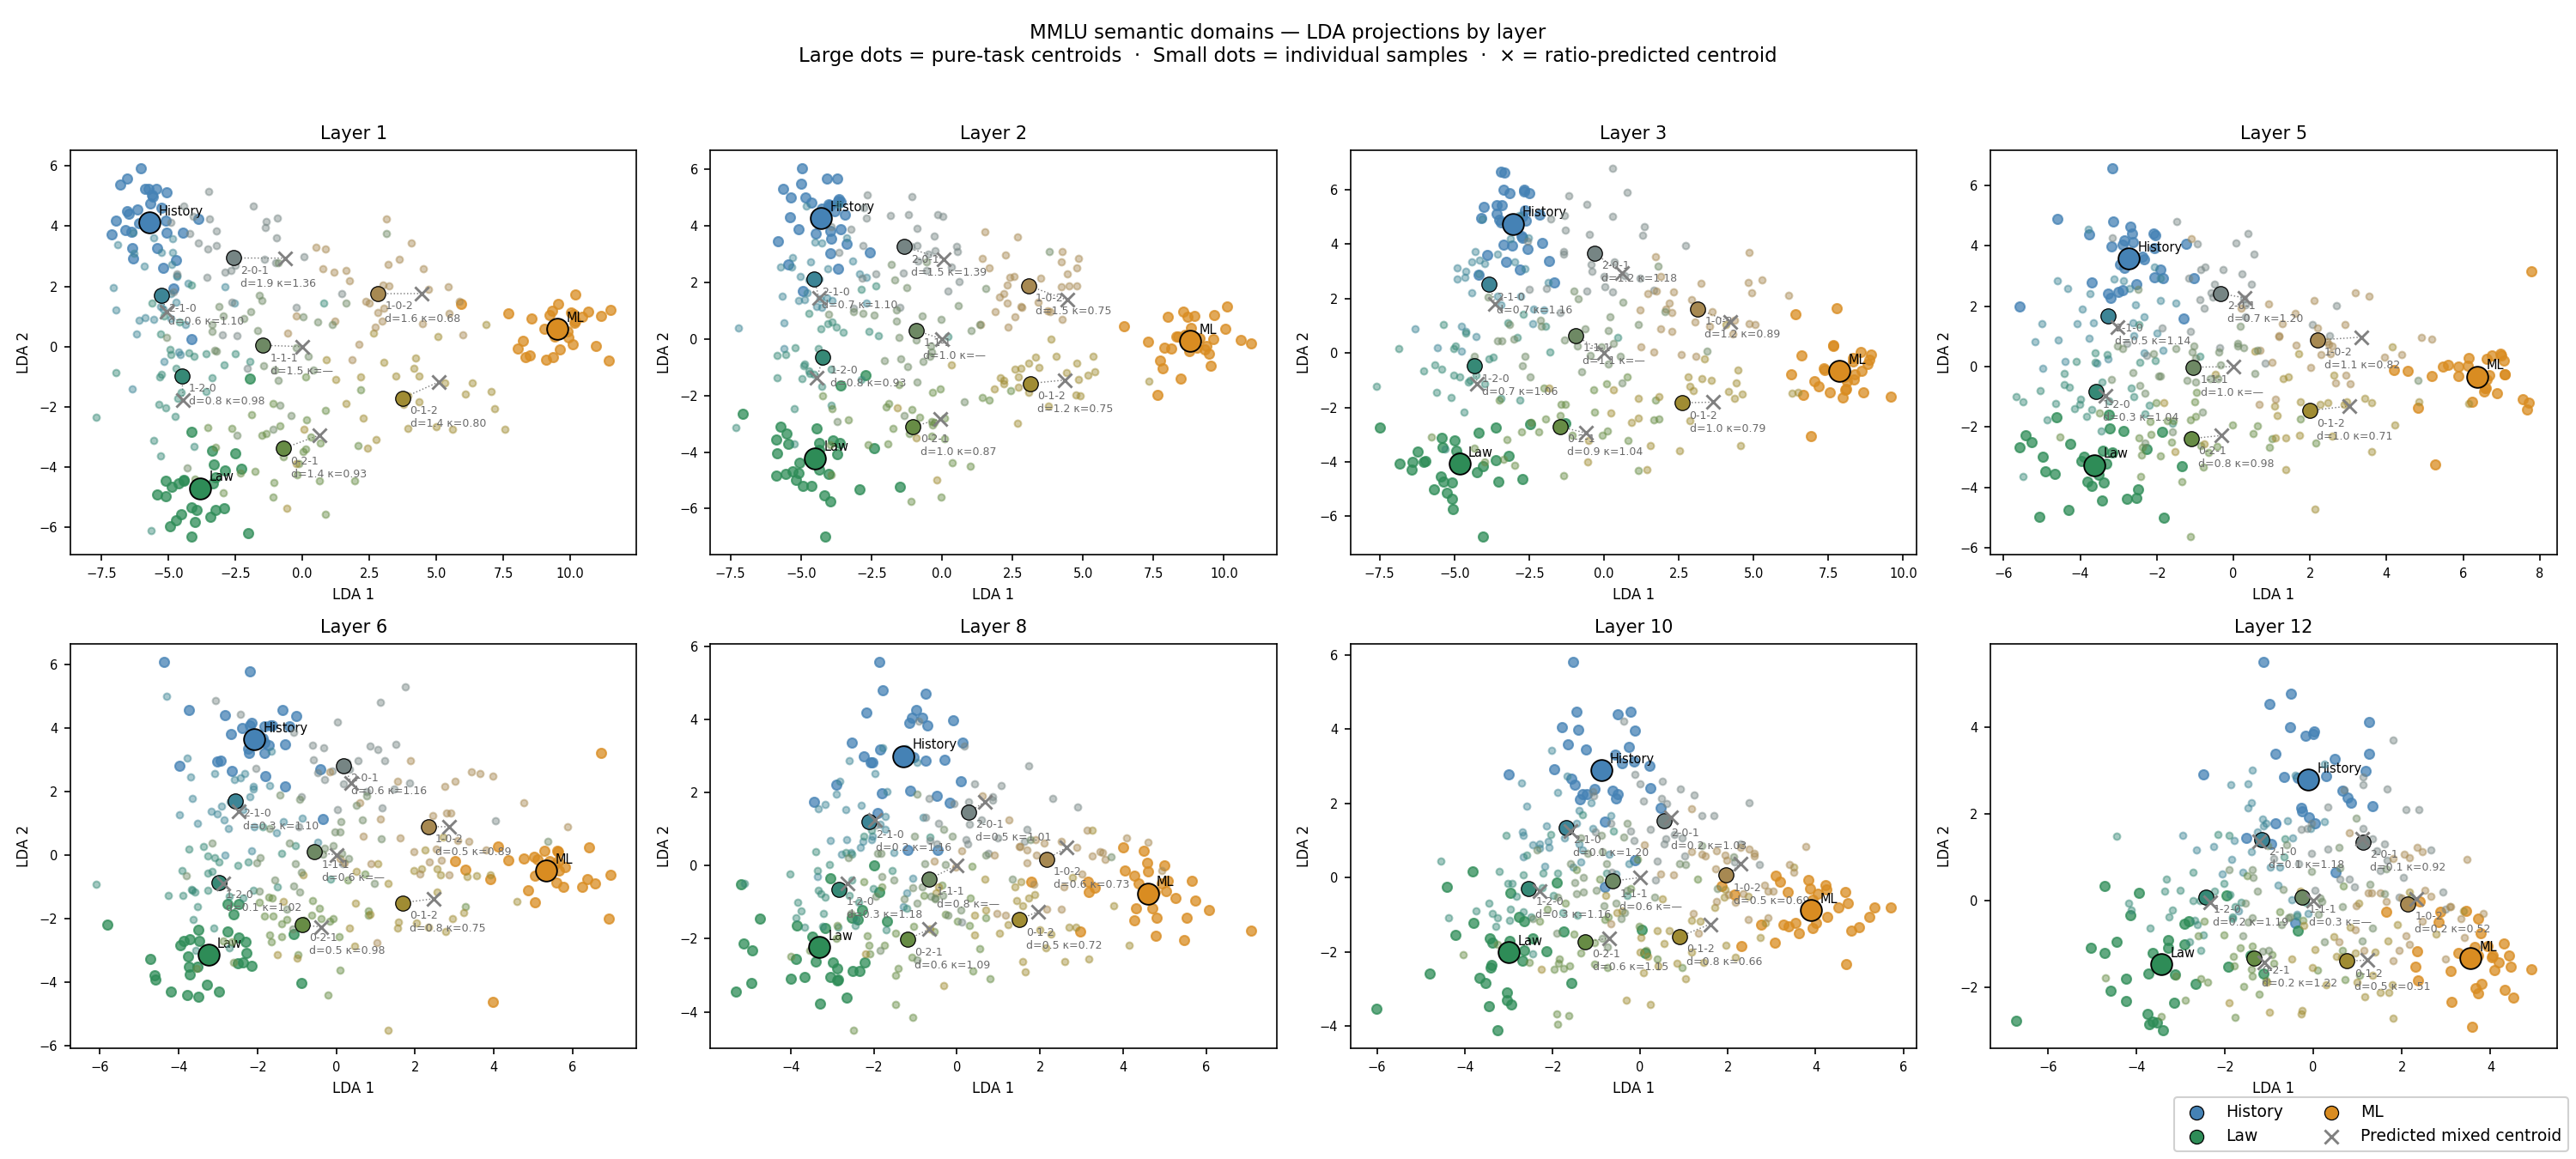
\includegraphics[width=\linewidth]{mmlu_layer_sweep_projections_Llama-1B_rotated.png}
        \caption{Llama 3.2 1B}
    \end{subfigure}
    \hfill
    \begin{subfigure}{0.48\linewidth}
        \centering
        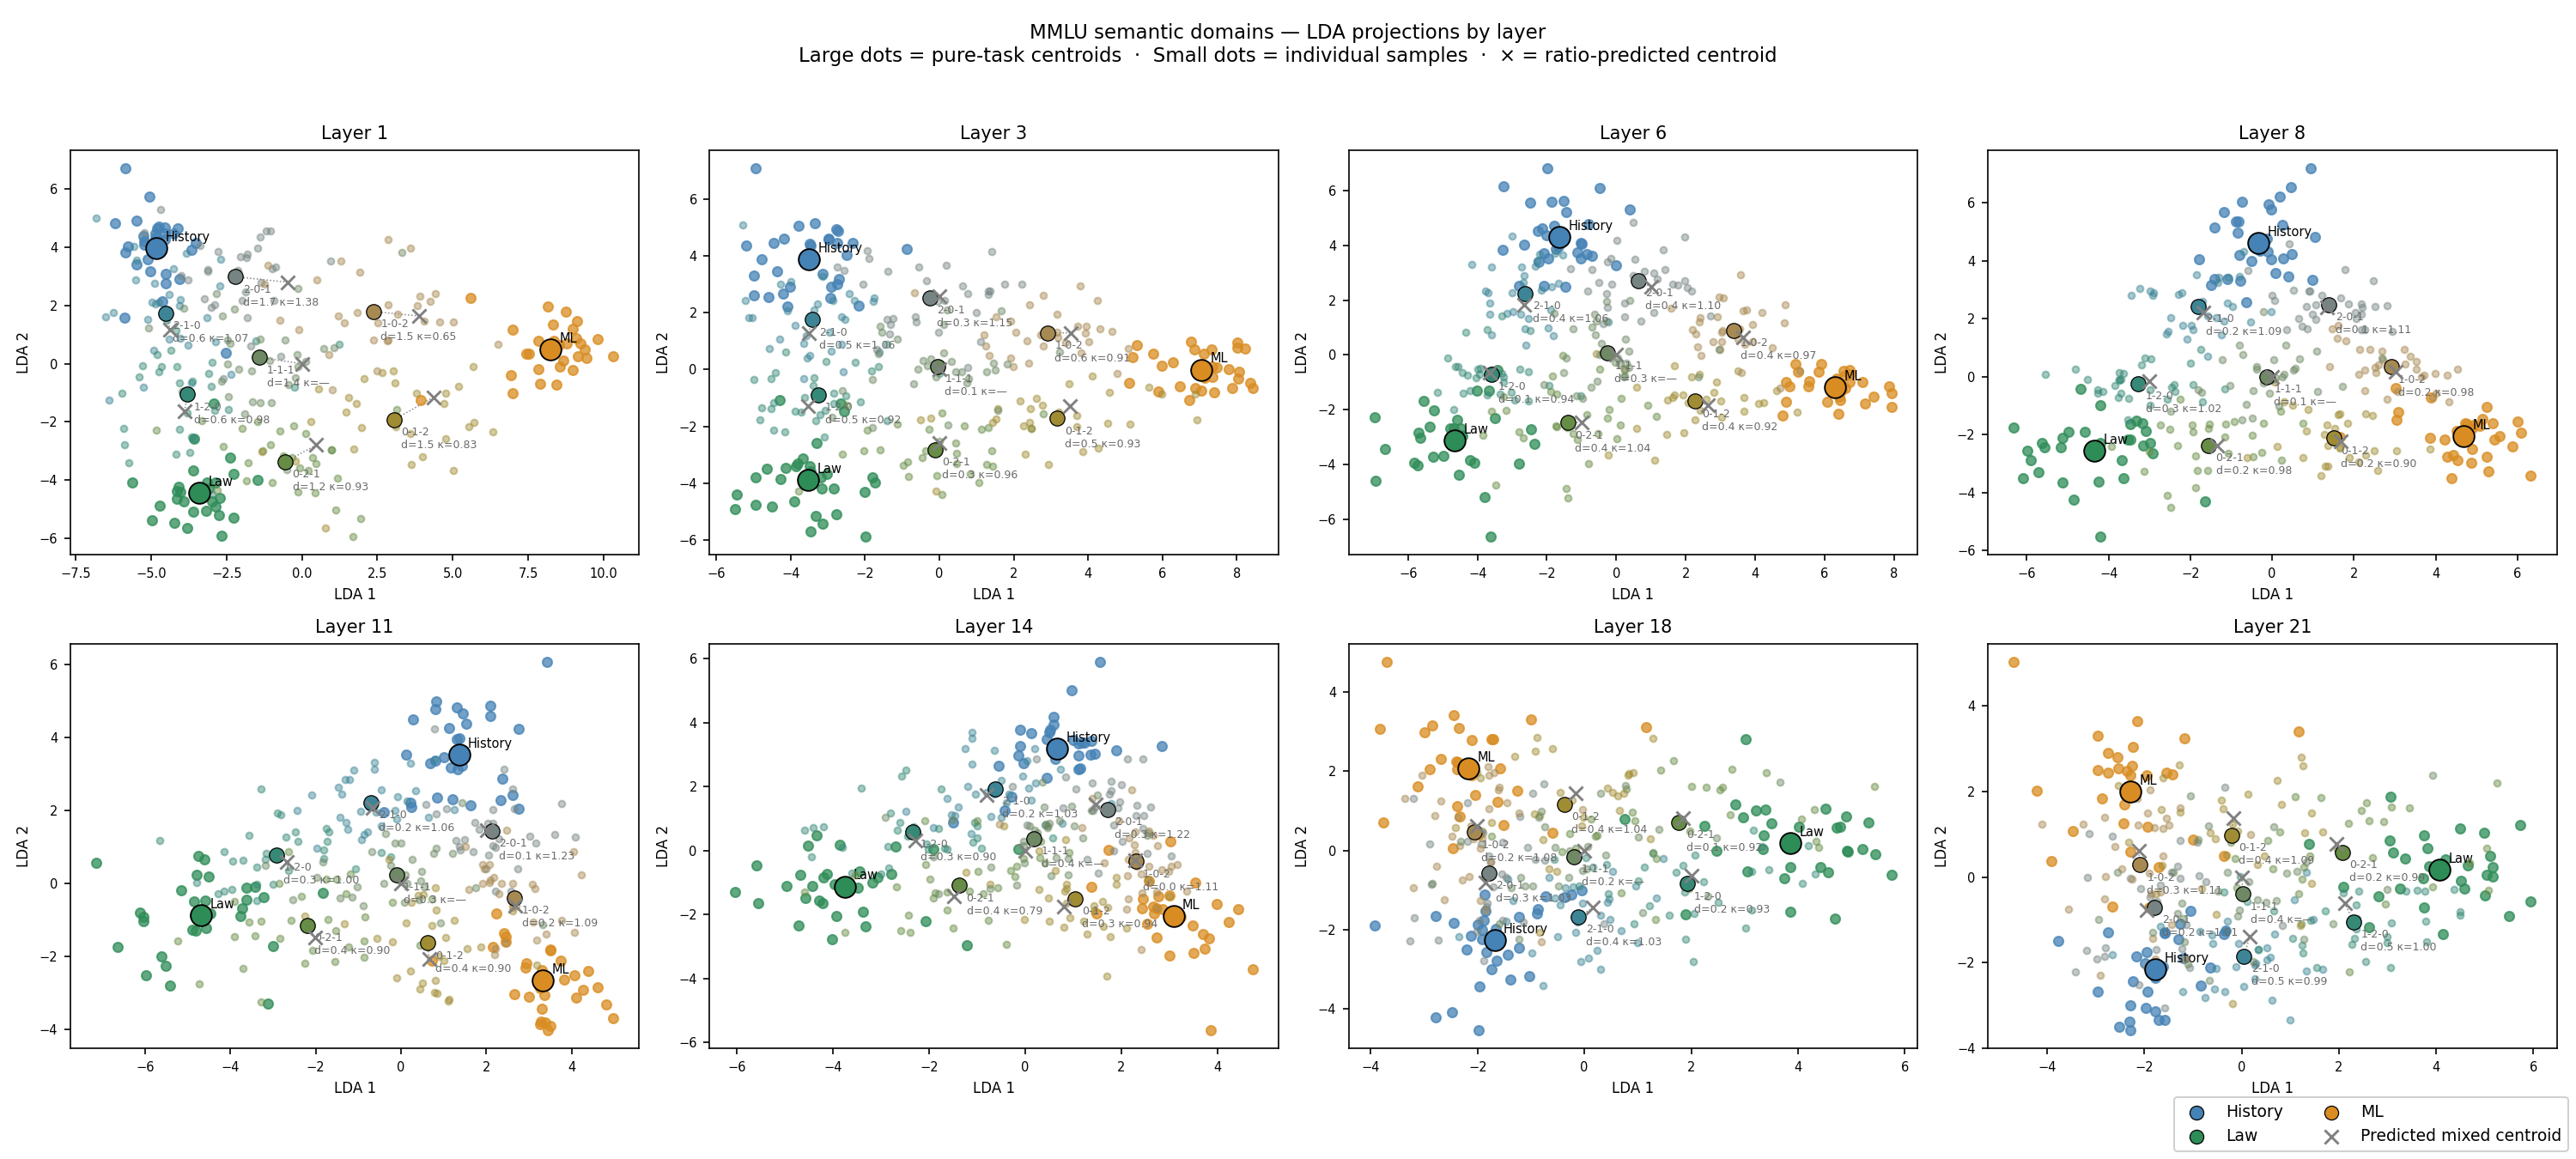
\includegraphics[width=\linewidth]{mmlu_layer_sweep_projections_Llama-3B_rotated.png}
        \caption{Llama 3.2 3B}
    \end{subfigure}

    \begin{subfigure}{0.48\linewidth}
        \centering
        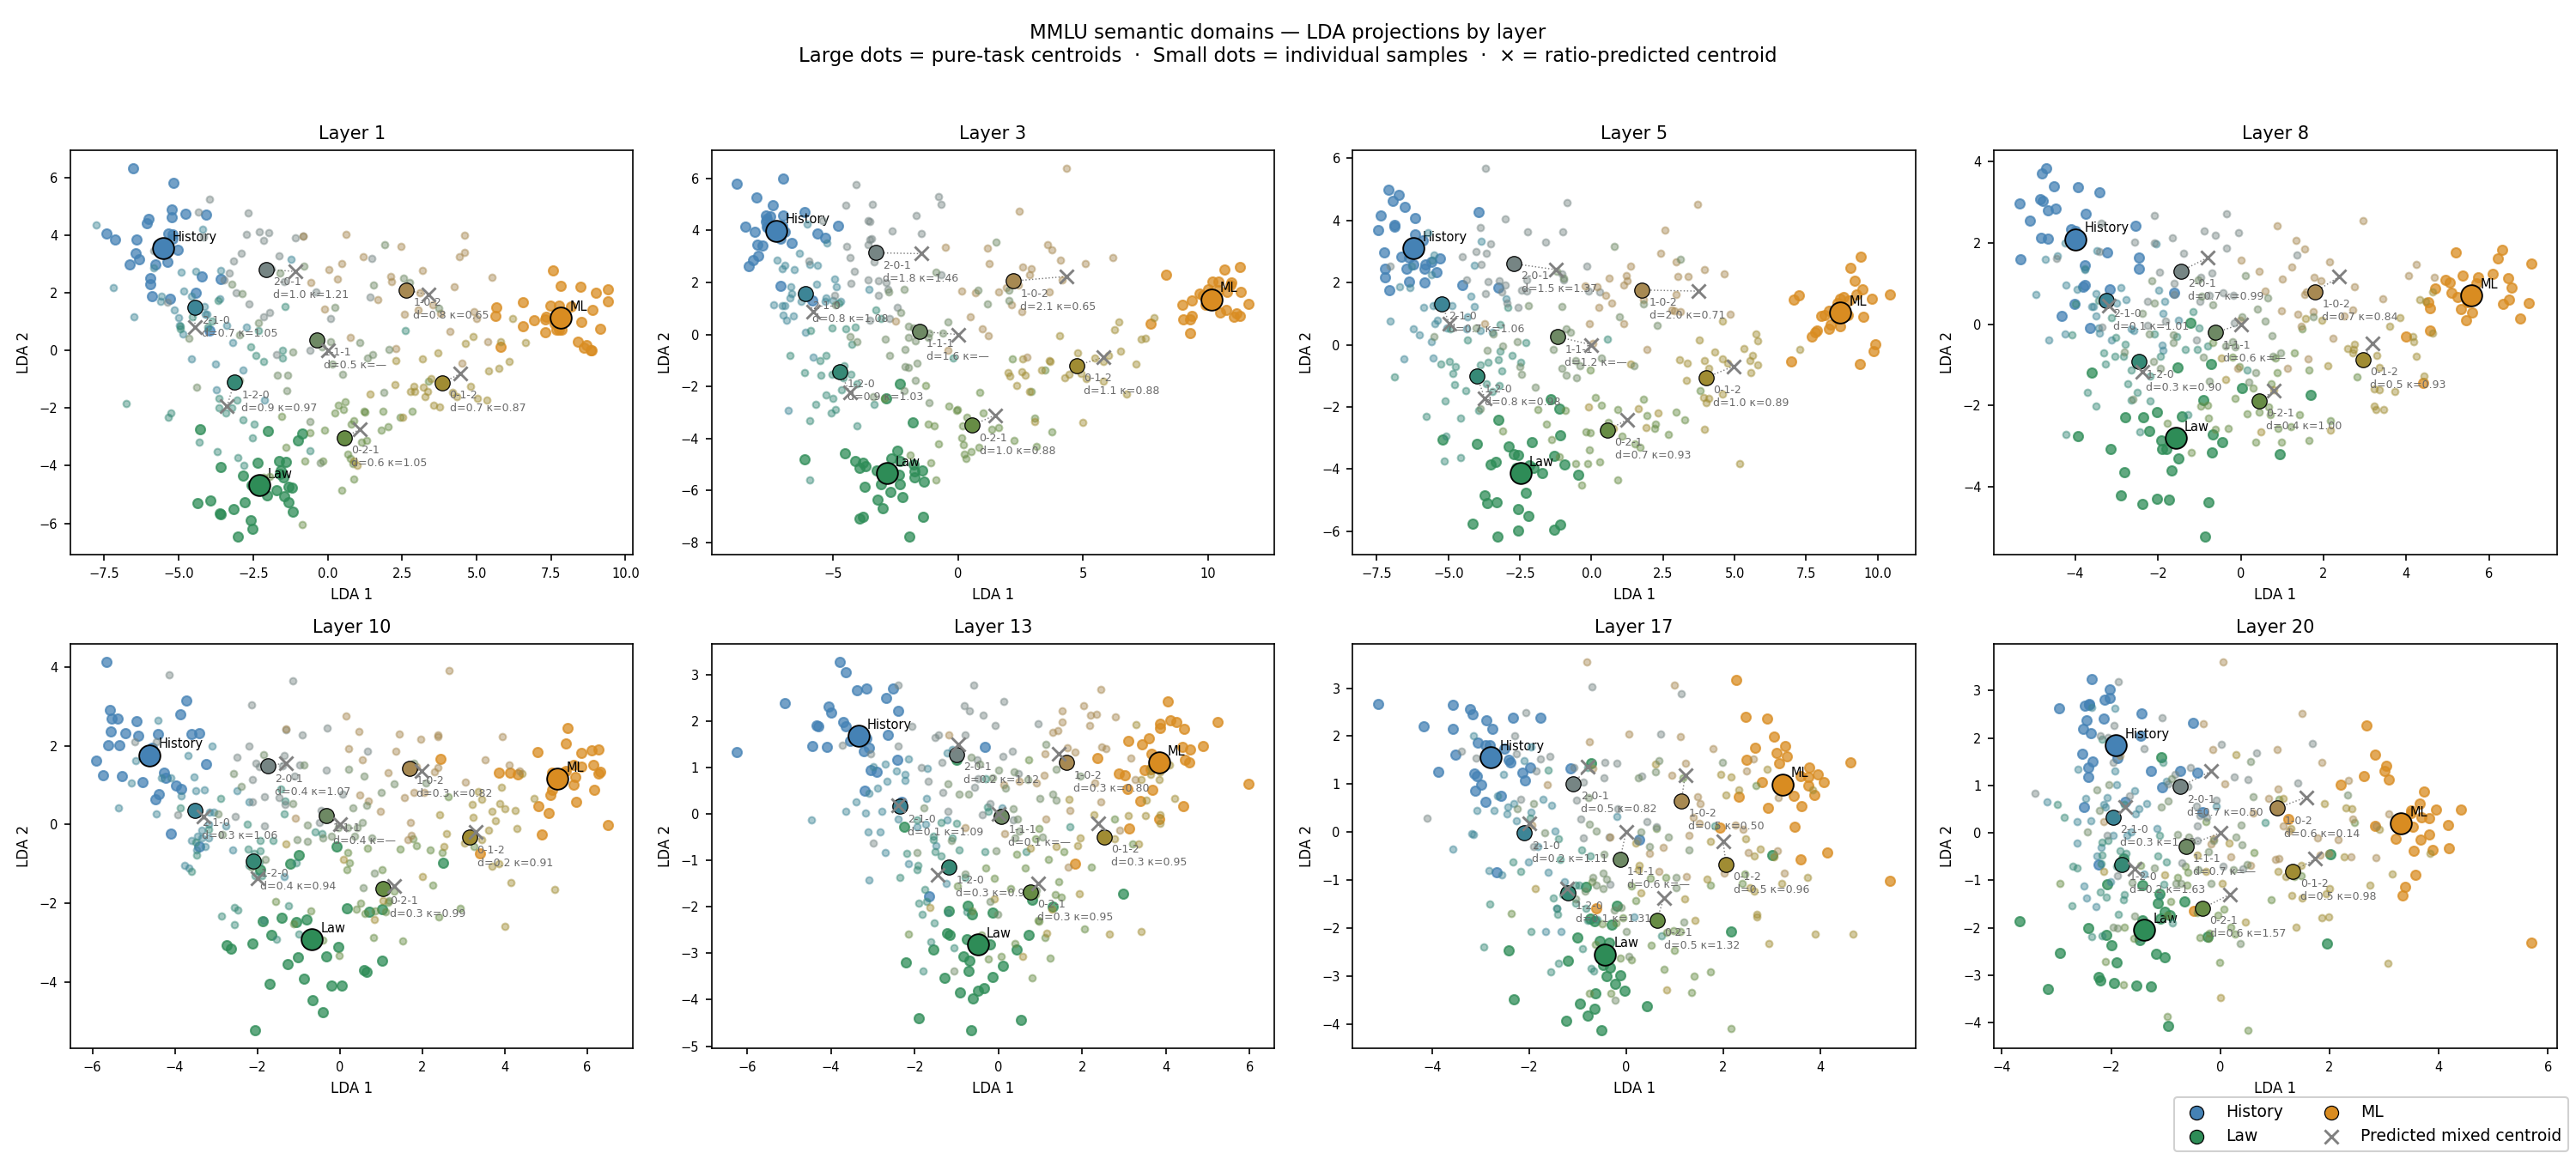
\includegraphics[width=\linewidth]{mmlu_layer_sweep_projections_Gemma-2B_rotated.png}
        \caption{Gemma 2 2B}
    \end{subfigure}
    \hfill
    \begin{subfigure}{0.48\linewidth}
        \centering
        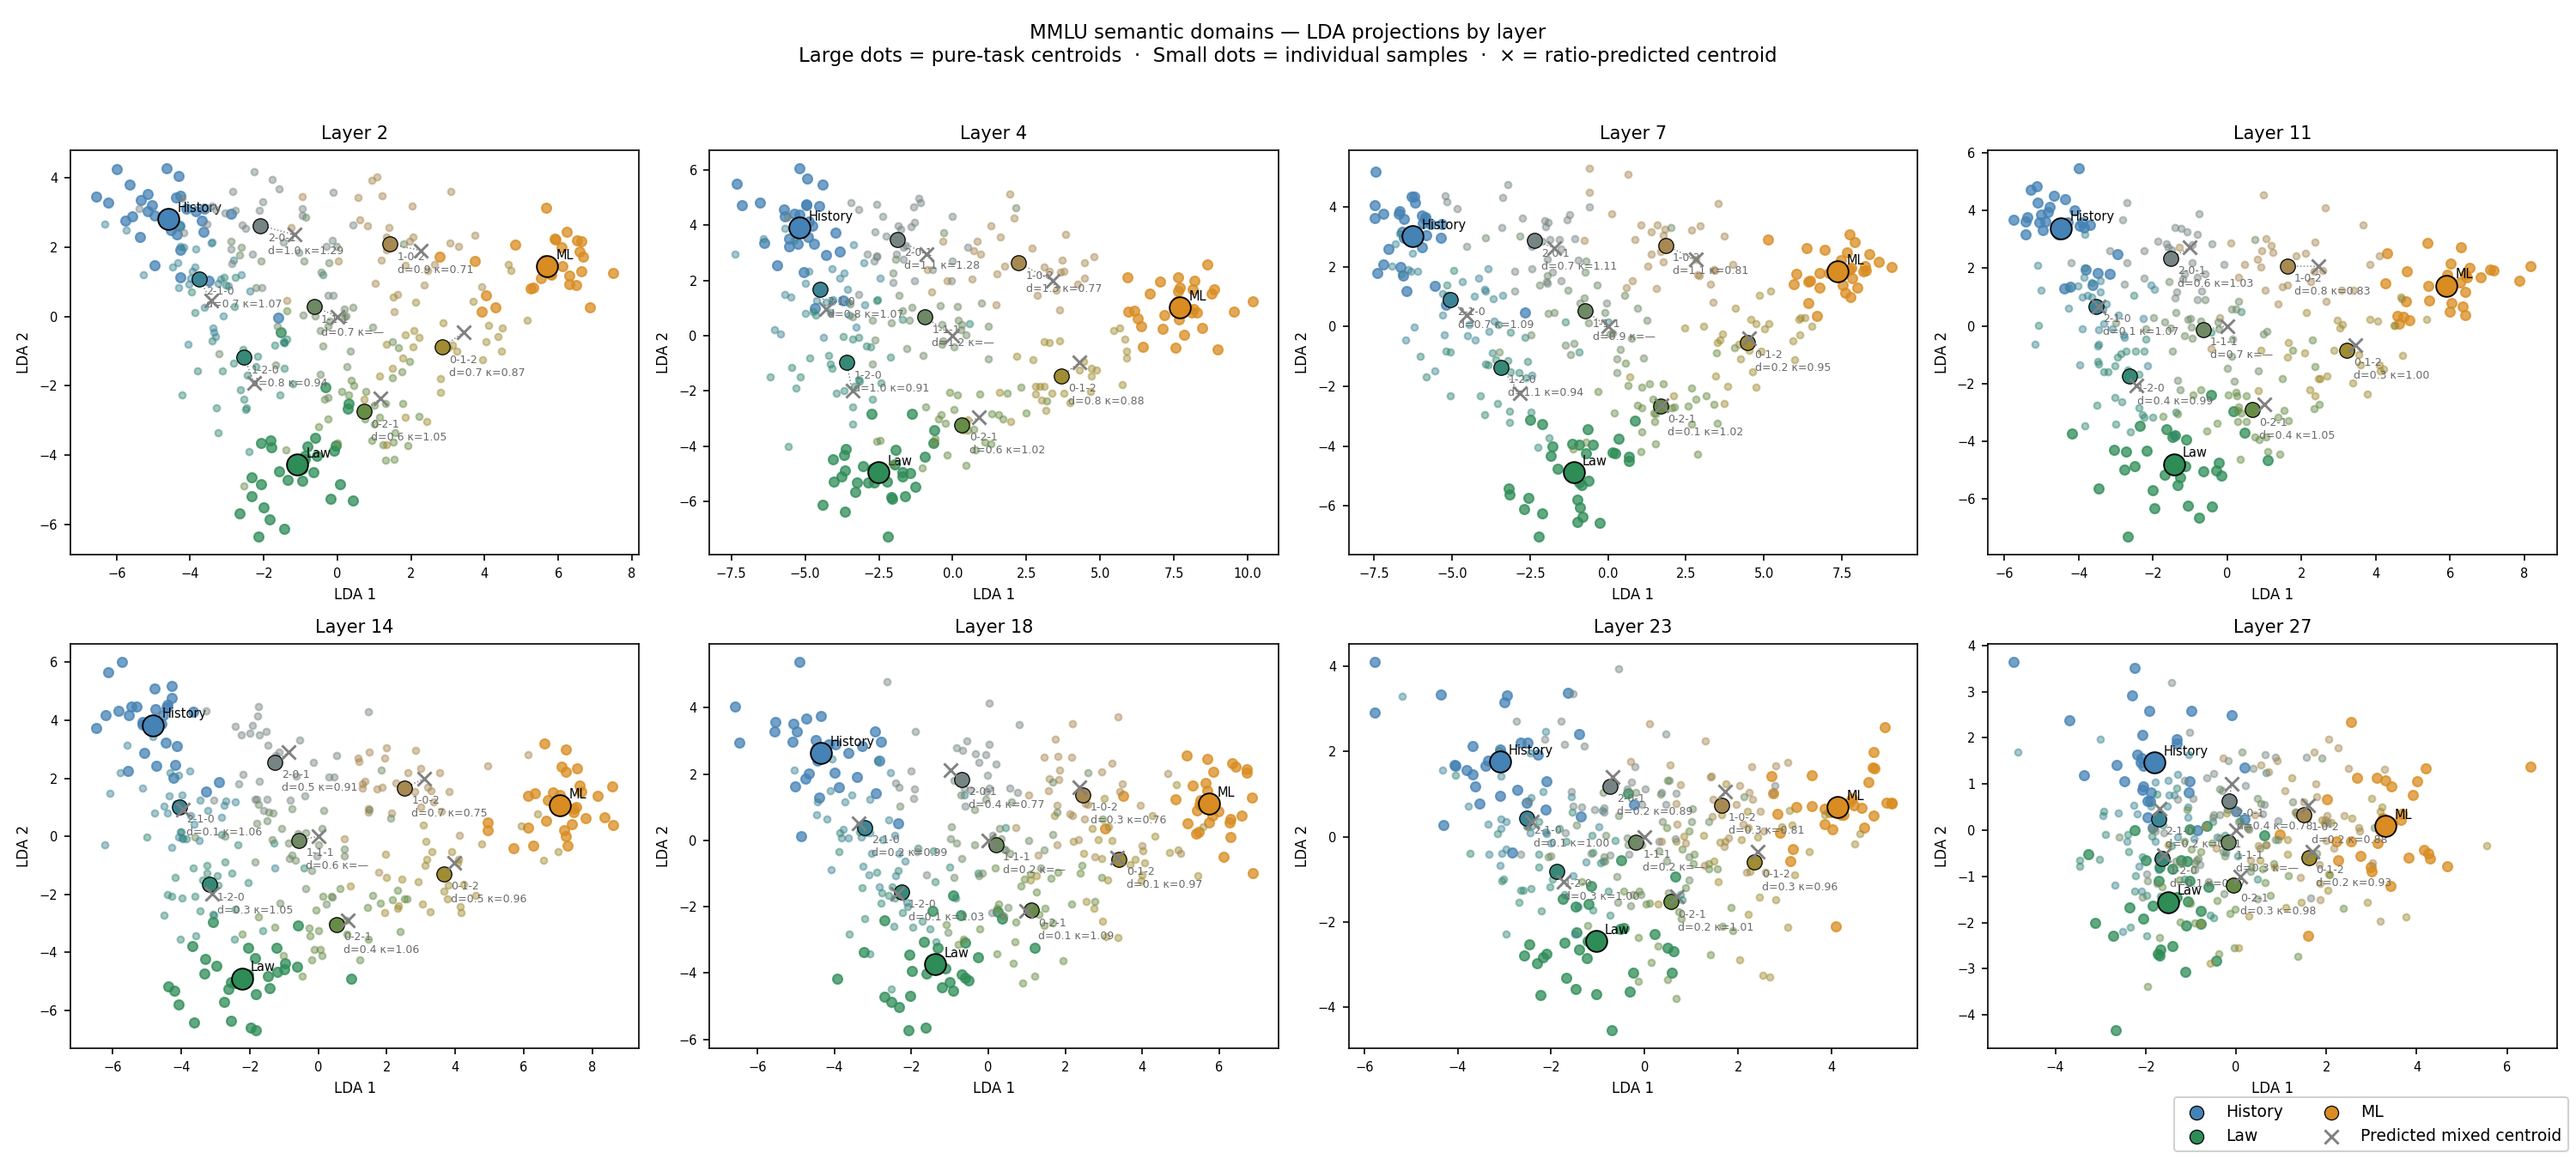
\includegraphics[width=\linewidth]{mmlu_layer_sweep_projections_Qwen-3B_rotated.png}
        \caption{Qwen 2.5 3B}
    \end{subfigure}
    \caption{MMLU layer sweep projections across models. \textbf{Colors:} Blue = History, Orange = ML, Green = Law. \textbf{Markers:} $\boldsymbol{\times}$~predicted centroid, $\bullet$~actual centroid for a ratio. *Llama 3.1 8B Instruct omitted due to hardware constraints}
    \label{fig:mmlu_results}
\end{figure}

\subsection*{Entity}
\begin{figure}[H]
    \centering
    \begin{subfigure}{0.48\linewidth}
        \centering
        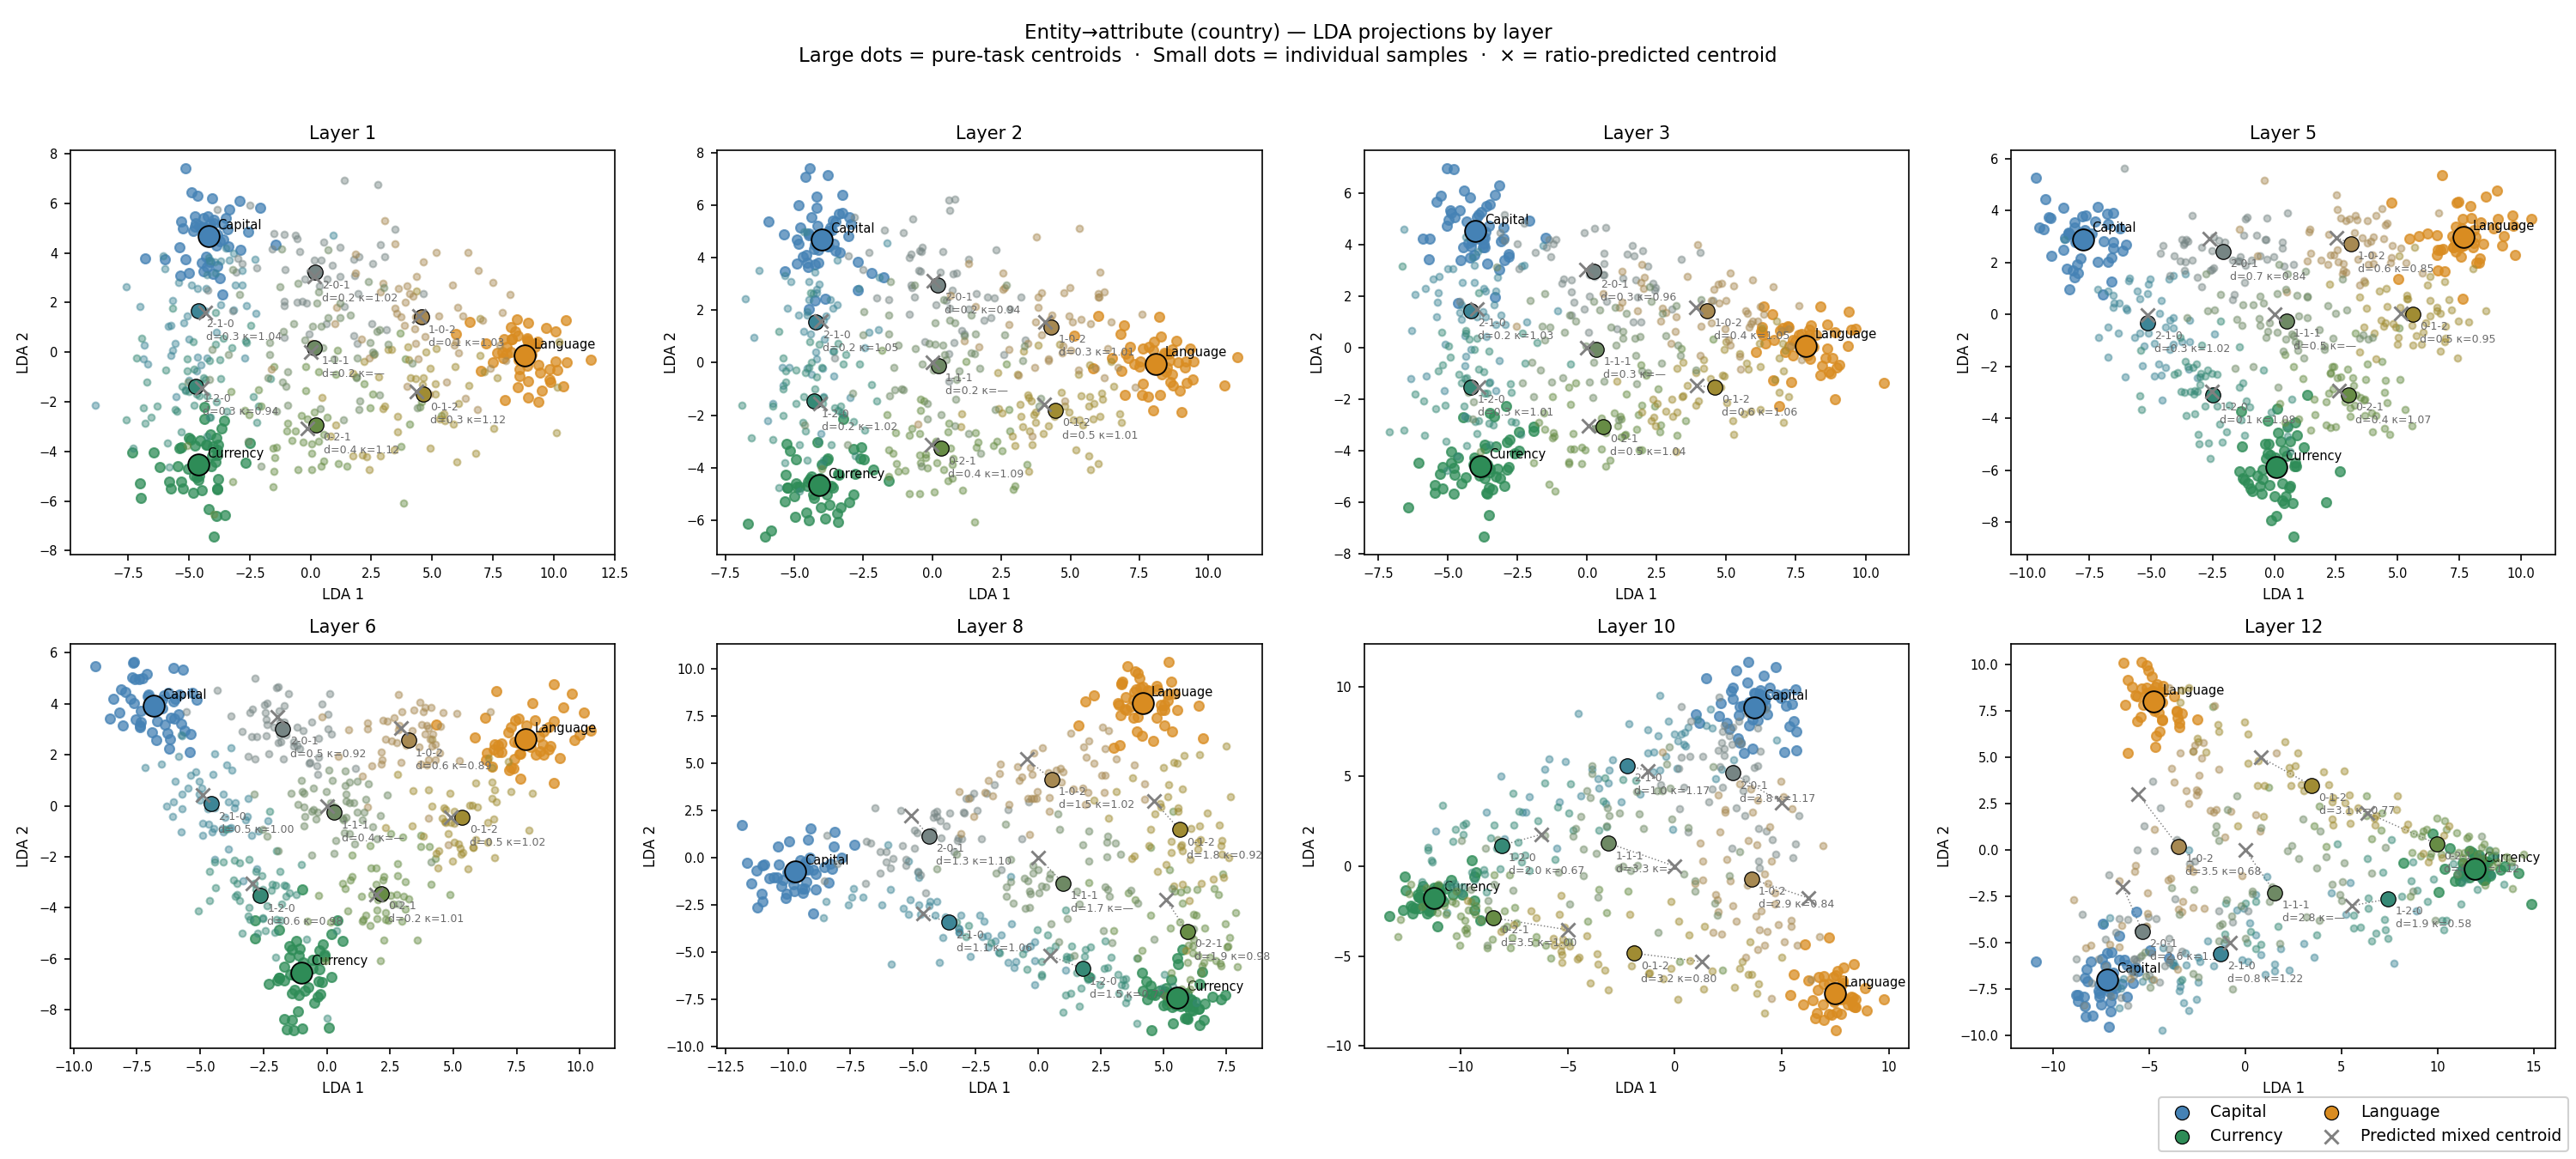
\includegraphics[width=\linewidth]{entity_layer_sweep_projections_Llama-1B_rotated.png}
        \caption{Llama 3.2 1B}
    \end{subfigure}
    \hfill
    \begin{subfigure}{0.48\linewidth}
        \centering
        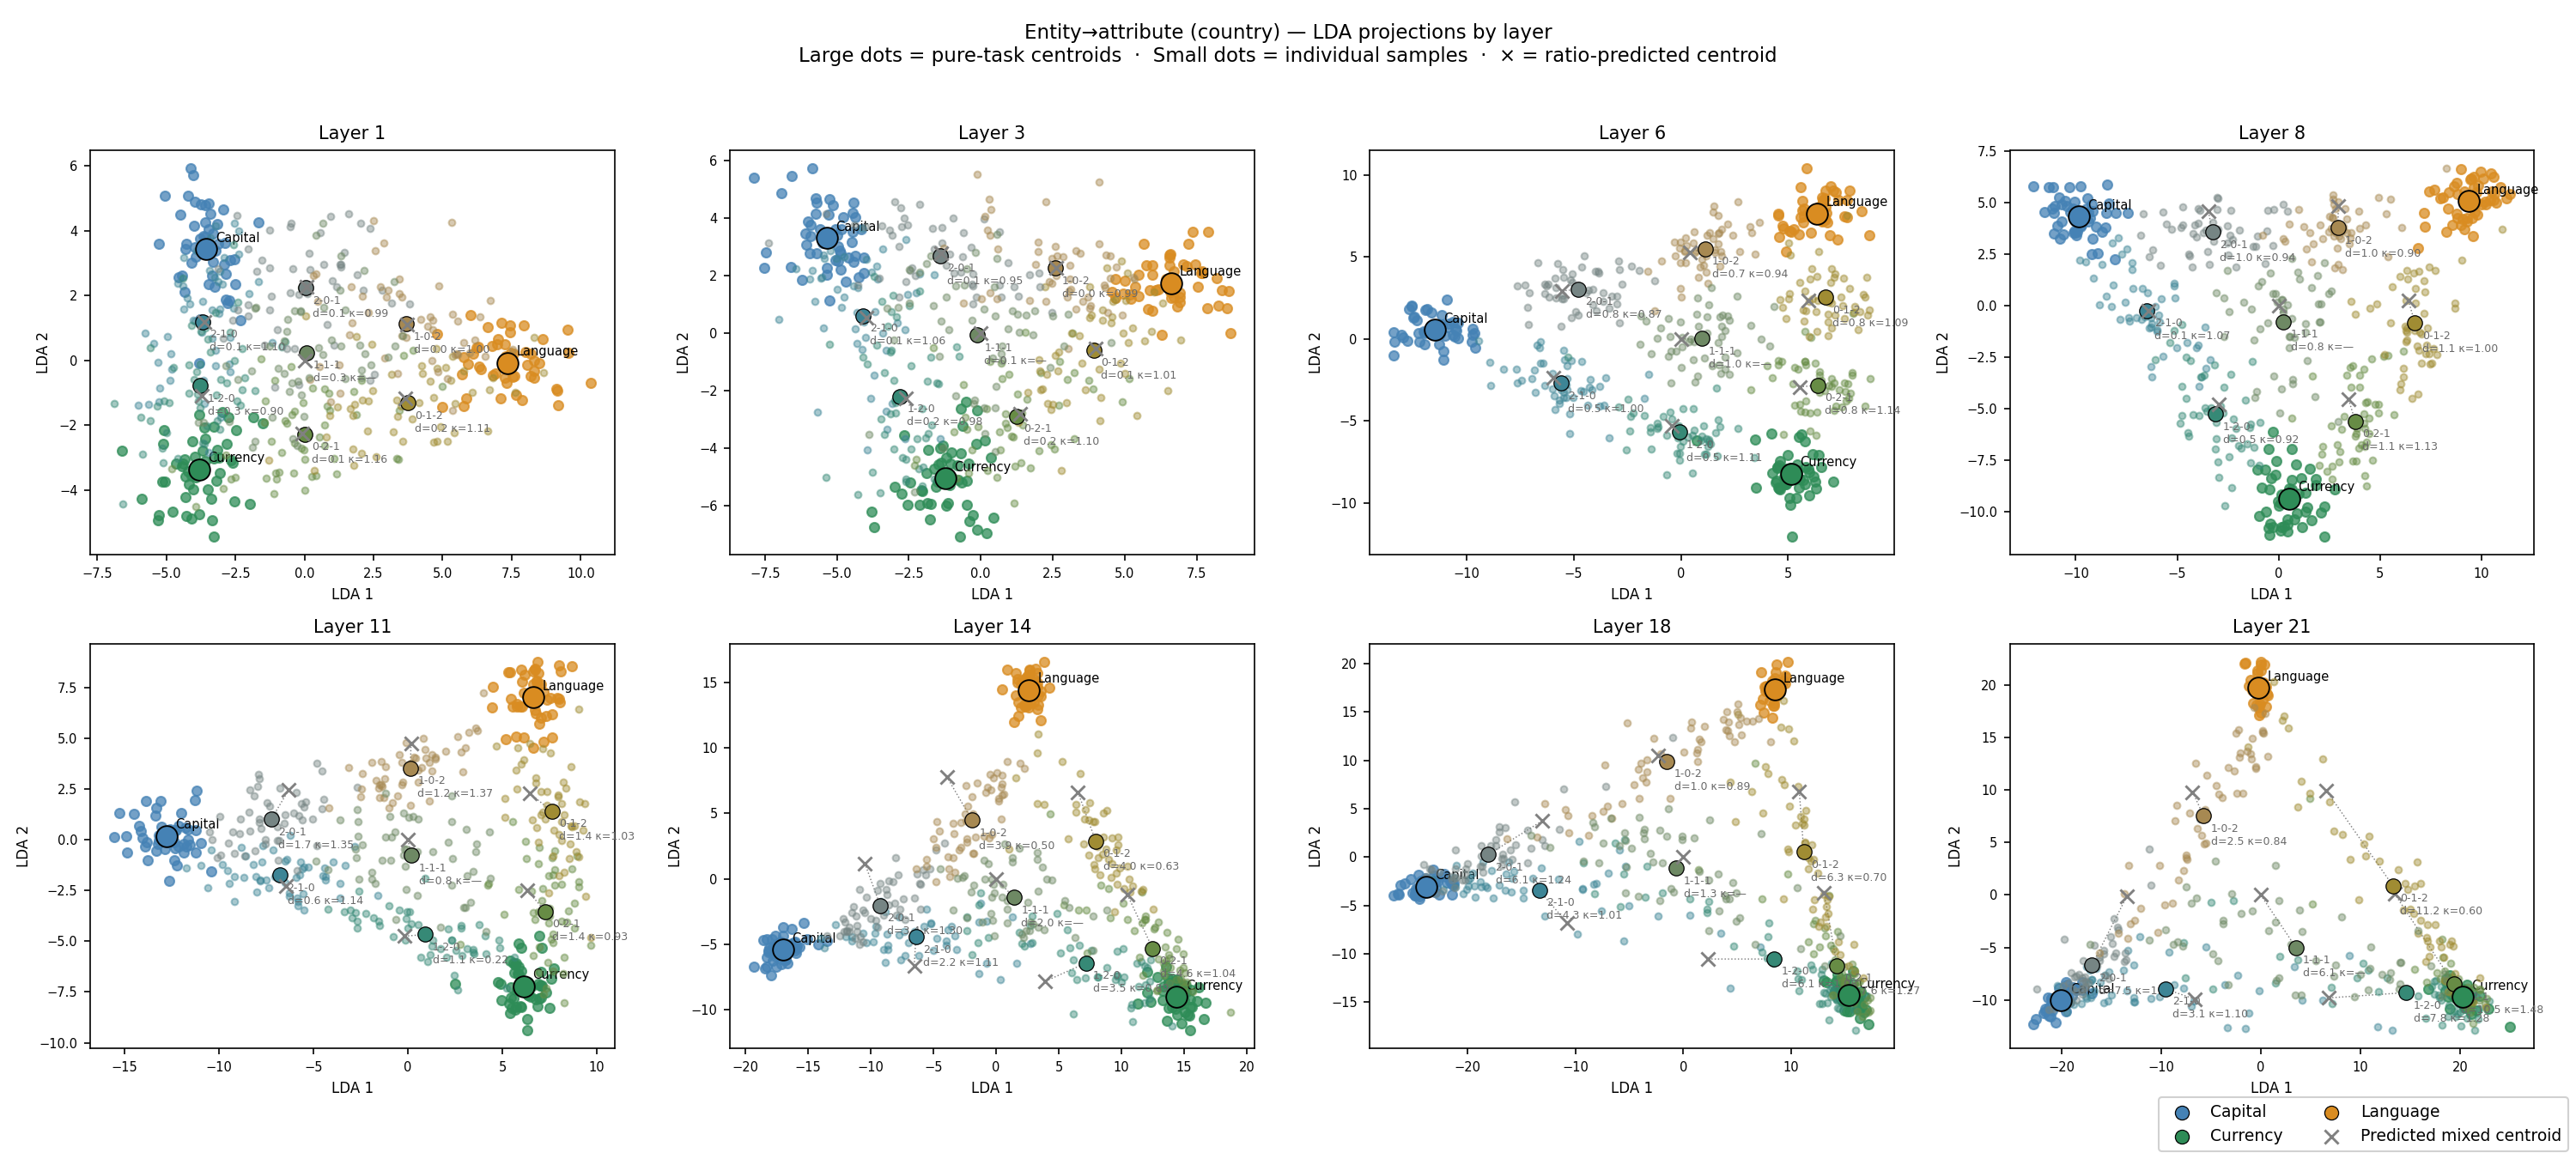
\includegraphics[width=\linewidth]{entity_layer_sweep_projections_Llama-3B_rotated.png}
        \caption{Llama 3.2 3B}
    \end{subfigure}
    \begin{subfigure}{0.48\linewidth}
        \centering
        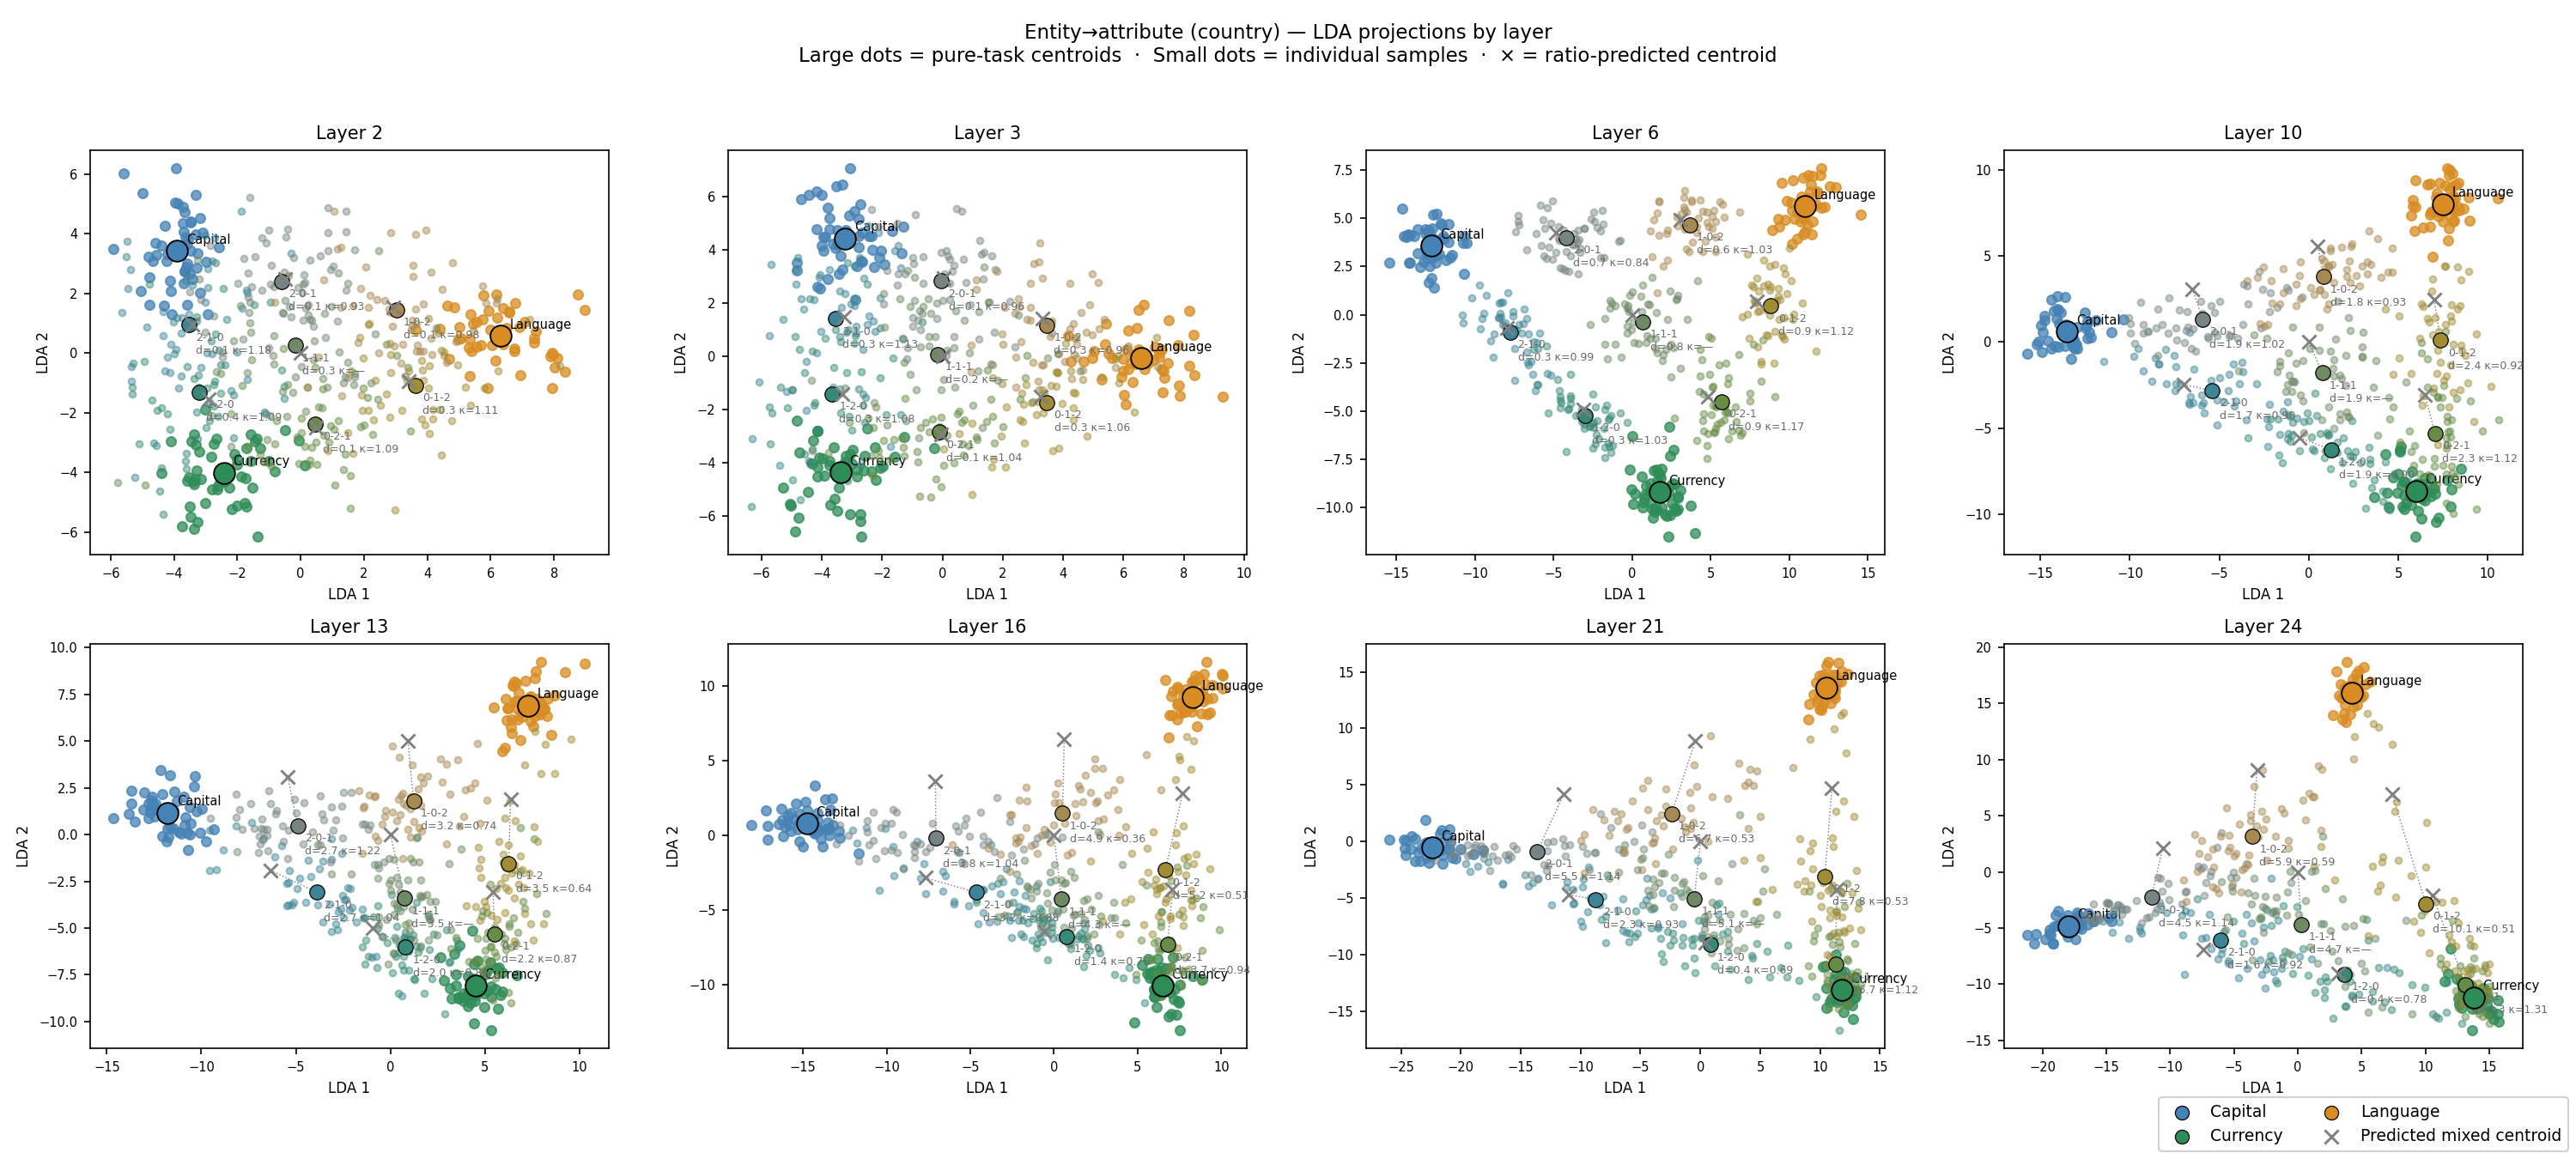
\includegraphics[width=\linewidth]{entity_layer_sweep_projections_Llama-8B_rotated.png}
        \caption{Llama 3.1 8B}
    \end{subfigure}
    \hfill
    \begin{subfigure}{0.48\linewidth}
        \centering
        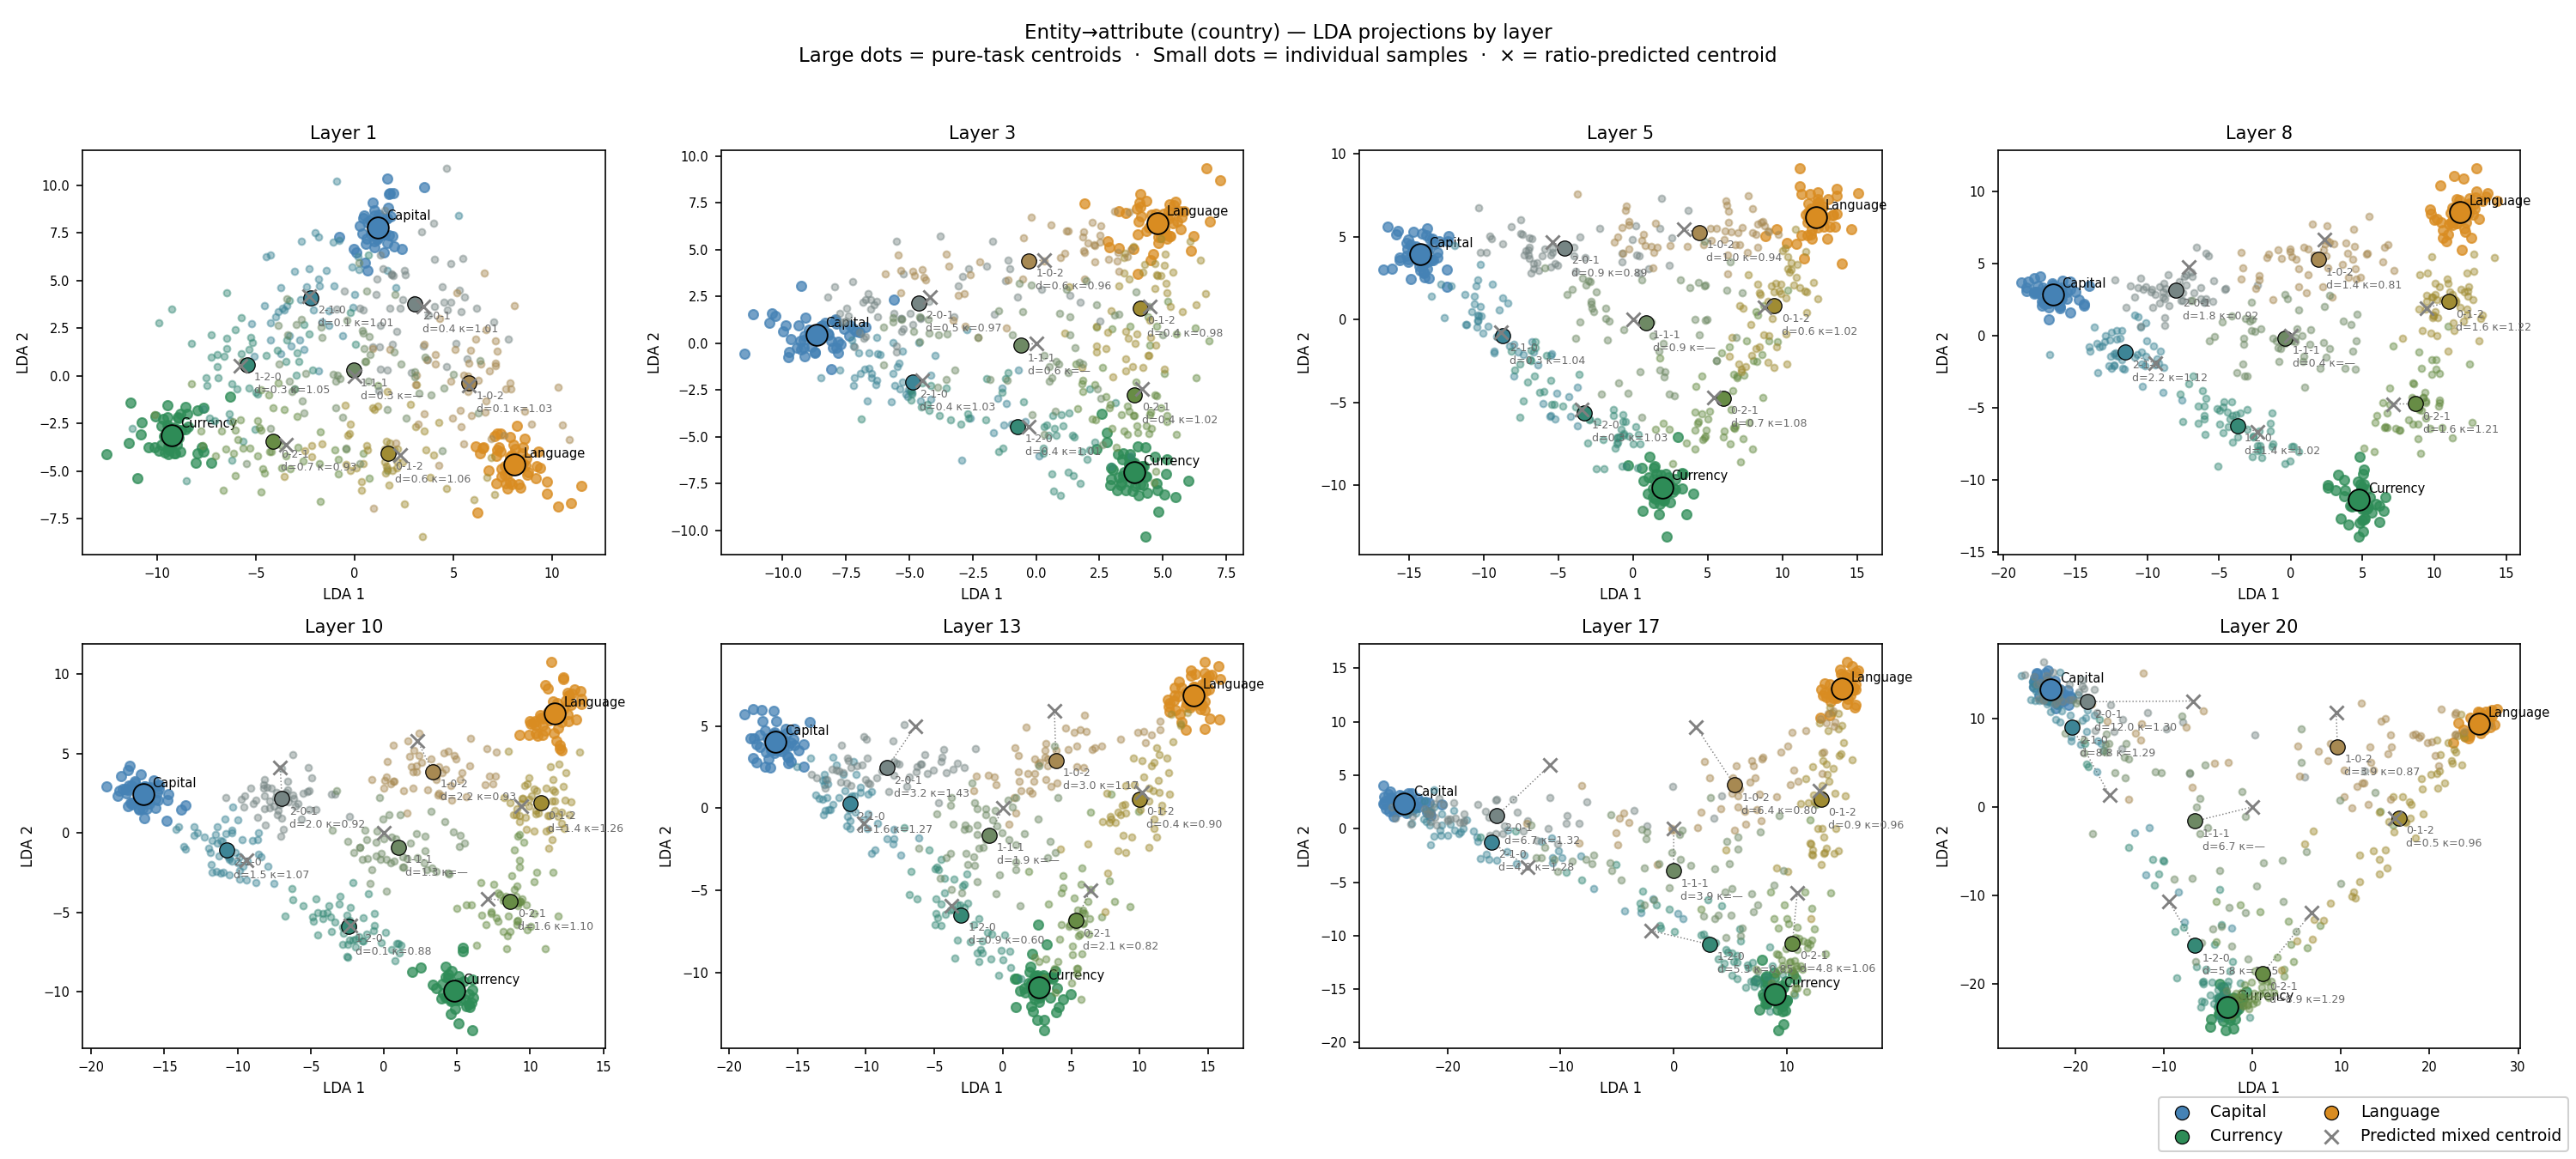
\includegraphics[width=\linewidth]{entity_layer_sweep_projections_Gemma-2B_rotated.png}
        \caption{Gemma 2 2B}
    \end{subfigure}

    \begin{subfigure}{0.48\linewidth}
        \centering
        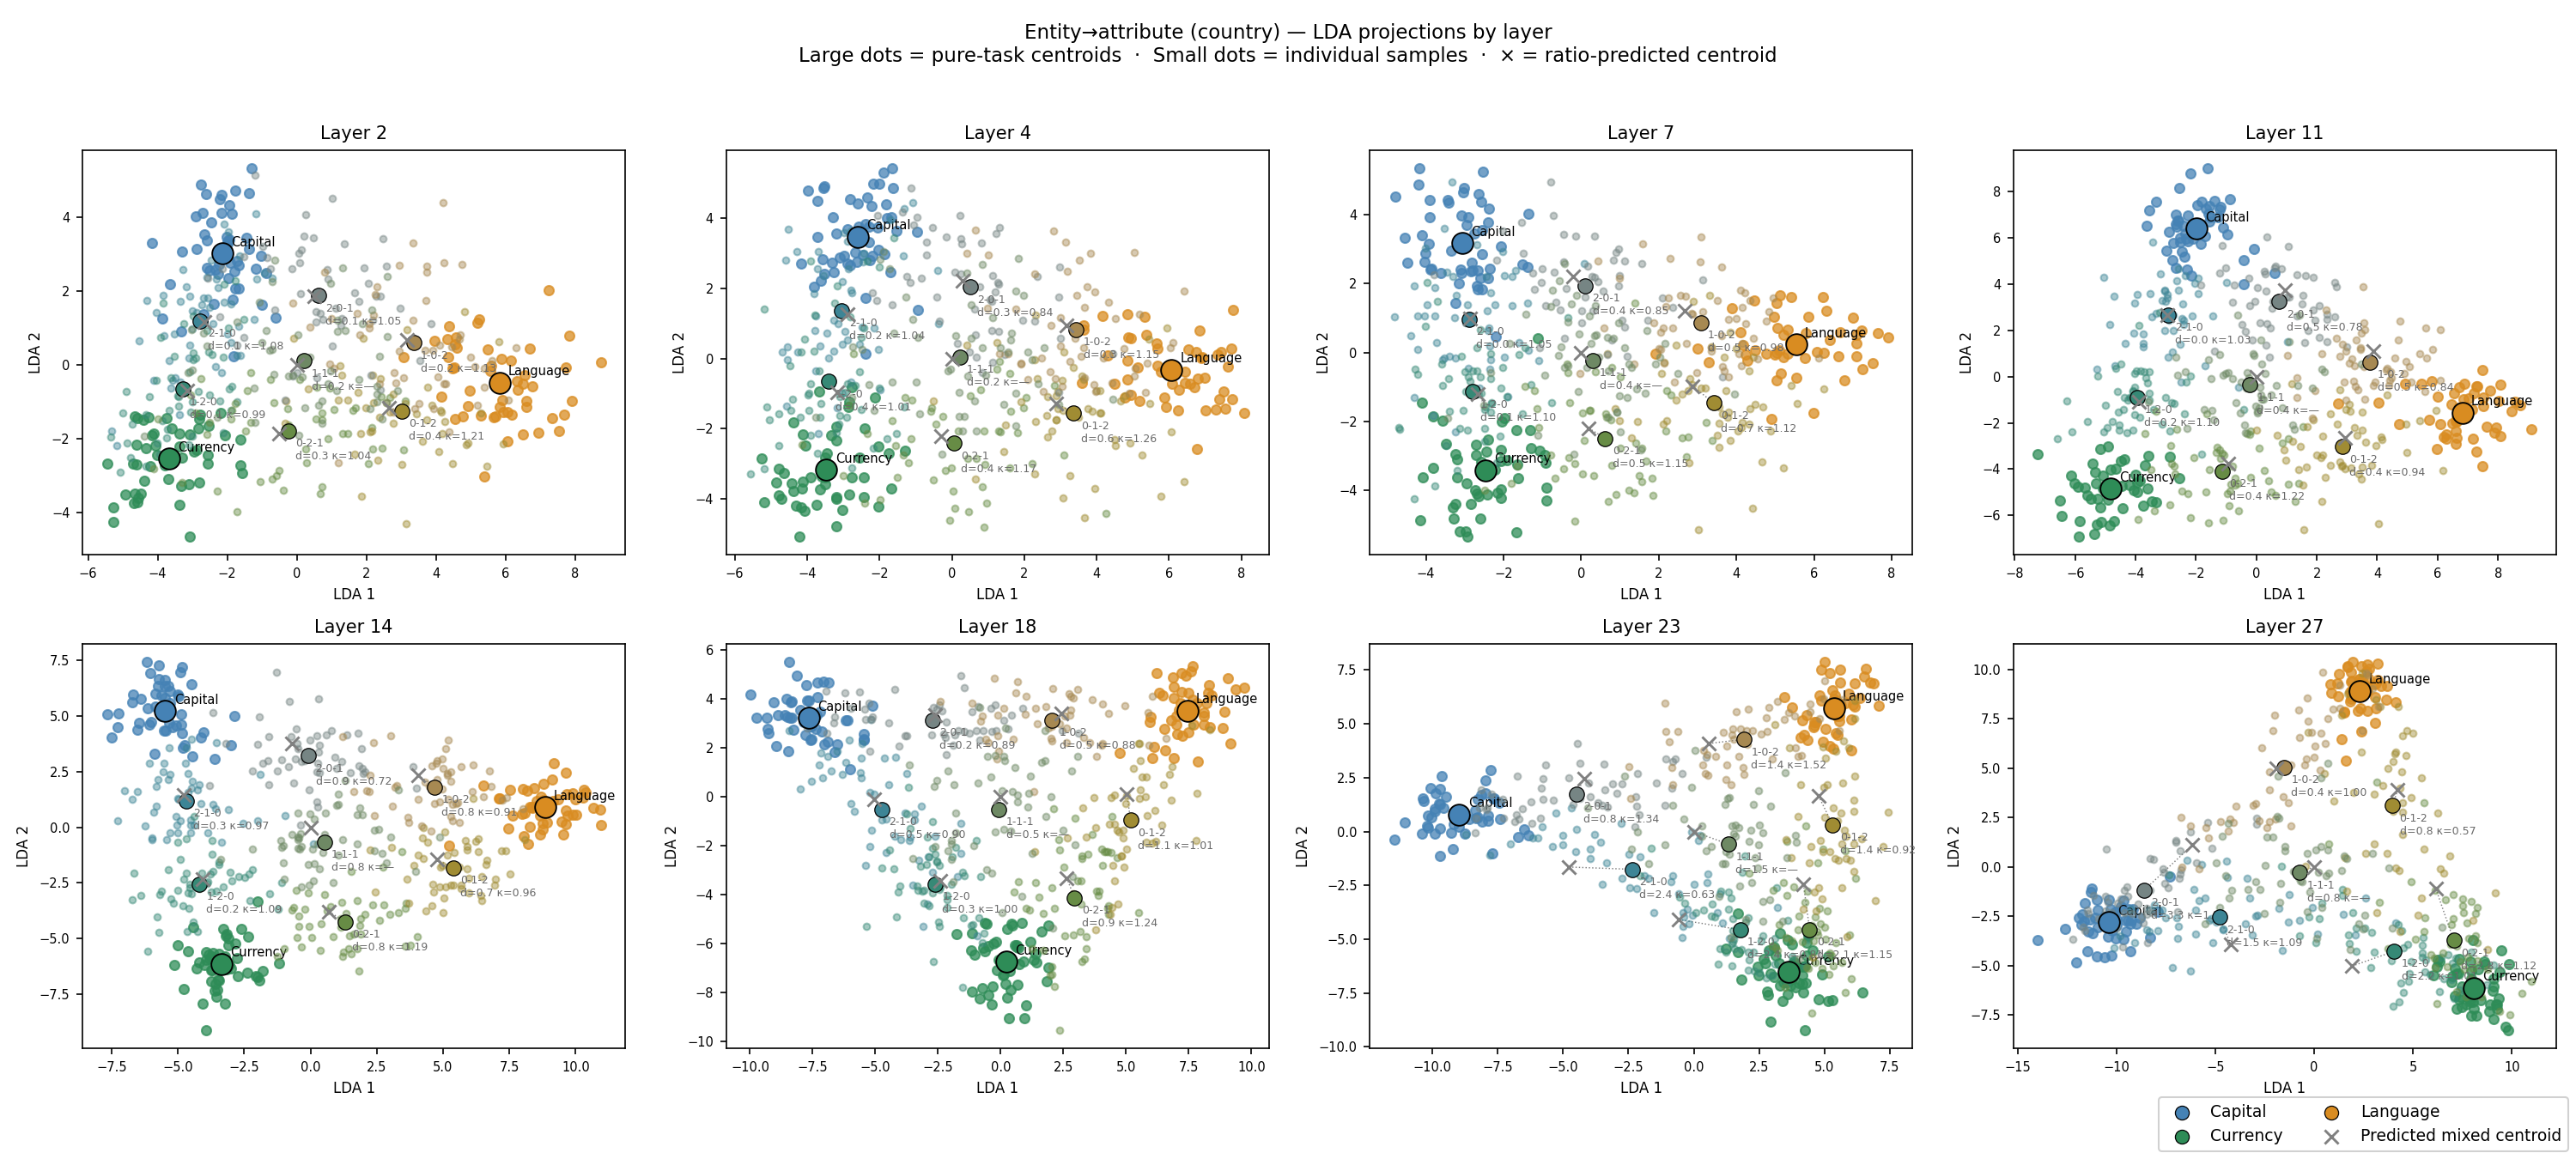
\includegraphics[width=\linewidth]{entity_layer_sweep_projections_Qwen-3B_rotated.png}
        \caption{Qwen 2.5 3B}
    \end{subfigure}
    \caption{Entity layer sweep projections across models. \textbf{Colors:} Blue = Capital, Orange = Language, Green = Currency. \textbf{Markers:} $\boldsymbol{\times}$~predicted centroid, $\bullet$~actual centroid for a ratio}
    \label{fig:entity_results}
\end{figure}

\section{OLS Closed form solution for \texorpdfstring{$\alpha_p$}{alpha p} coefficients}
\label{appendix:ols_sol}
As defined in \ref{subsec:kappa}, let \(\mu_p^l := \frac{1}{n} \sum_{i = 1}^n \textbf{c}_p^l (x_i)\), be the precomputed contrast vector centroid for a pure task ratio \(p \in P\) and \(\textbf{c}_r^l(x)\) be the contrast vector with test question \(x\) and in-context ratio \(r\), both extracted at layer \(l\). Let \(\alpha_1 \ldots \alpha_{|P|}\) be the mixing coefficients for the contrast vector centroids such that \(\sum_{p \in P} \alpha_p \mu_p^l\) is the OLS estimate for \(\textbf{c}_r^l\) under the constraint \(\sum_{p \in P} \alpha_p = 1\). We investigate how we can recover all \(\alpha_p\) and show that these coefficients (i) are non-negative and (ii) resemble the task ratio \(r\) in the original prompt. \\[1em]
In order to enforce \(\sum_{p \in P} \alpha_p = 1\), we reparameterize the \(\alpha_p\)s and set the last coefficient \(\alpha_{k} = 1 - \sum_{p \in P \setminus \{k\}} \alpha_p\), giving \(|P| - 1\) covariates. \\[1em]
We can thus express the reparameterized linear combination as 
$$
    \sum_{p \in P \setminus \{k\}} \alpha_p \mu_p^l + \left(1 -  \sum_{p \in P \setminus \{k\}}\alpha_p\right) \mu_k^l = \textbf{c}_r^l
$$
and solve for the \(\alpha_p\)s in this new system. Since each contrast vector and pure task centroid is in \(\mathbb{R}^d\) where \(d \gg |P|\), the system is overdetermined. Hence, we can use least squares to solve this system, treating each dimension of the pure task centroids as a datapoint. \\[1em]
From this, we see that
\begin{align*}
    &\sum_{p \in P \setminus \{k\}} \alpha_p \mu_p^l + \left(1 -  \sum_{p \in P \setminus \{k\}}\alpha_p\right) \mu_k^l = \textbf{c}_r^l \\[1em]
    &\implies \sum_{p \in P \setminus \{k\}} \alpha_p  (\mu_p^l - \mu_k^l) + \mu_k^l = \textbf{c}_r^l \\[1em]
    &\implies \sum_{p \in P \setminus \{k\}} \alpha_p  (\mu_p^l - \mu_k^l) = \textbf{c}_r^l - \mu_k^l 
\end{align*}
where the pure task centroids \(\mu_p^l\) and test contrast vector \(\textbf{c}_r^l\) are in \(\mathbb{R}^d\) and there are \(|P| - 1\) \(\alpha\) coefficients. \\[1em]
From this, we see that the design matrix \(X\) is a \(d \times (|P| - 1)\) matrix with \(\mu_k^l\) subtracted from each of the first \(|P| - 1\) pure task centroids as column vectors:
$$
    X := \begin{bmatrix}\mu_{p_1}^l - \mu_k^l & \mu_{p_2}^l - \mu_k^l & \ldots & \mu_{p_{|P| - 1}}^l - \mu_k^l\end{bmatrix}
$$
and the response vector \(y\) is \(\textbf{c}_r^l - \mu_k^l\). We can also stack the coefficients \(\alpha_{p_1} \ldots \alpha_{|P| - 1}\) in a column vector \(\alpha \in \mathbb{R}^{|P| - 1}\). This gives us the final system of equations \(y = X \alpha\) that we can solve through OLS. \\[1em]
From this, we see that the closed form solution for \(\alpha\) is 
$$\hat\alpha = (X^\top X)^{-1} X^\top y$$
and the last pure task coefficient is 
$$\hat \alpha_k = 1 - \sum_{p \in P\setminus\{k\}} \hat\alpha_p$$

\subsection*{Baseline comparison}
To demonstrate that the coefficients recovered by using the pure task centroids recover the ratio due to task-specific information, we compare the \(\alpha\) values recovered through reparameterized OLS using (i) pure task centroids and (ii) the common component (arithmetic mean) of the pure task centroids with added Gaussian noise. Specifically, we test $H_0:$ noise centroids recover the true weights as well as pure centroids (recovery is task-agnostic). \\[1em]
We construct noise centroids that preserve the shared structure of the pure centroids while destroying their task-specific directions. Let \(\bar \mu^l := \frac{1}{|P|} \sum_{p \in P} \mu_p^l\) be the common component of pure task centroids at layer \(l\). For each task p, we compute its residual \(\mu^l_p - \bar \mu^l\) draw a Gaussian vector \(v \sim N(\b0_d, I_d)\) and add \(||\mu^l_p - \bar \mu^l|| \frac{v^l}{||v^l||}\) to \(\bar \mu\) to get the noise centroid corresponding to pure ratio \(p\). The resulting noise centroids match the pure centroids in their common component and per-task residual norm, differing only in the residual direction. Hence, any drop in recovery quality is attributable to the loss of task-specific geometry. \\[1em]
To conduct this test, we use the  L2 distance of the coefficients from their expected values. For each ratio \(r\), the null distribution is obtained from the L2 norms of the recovered coefficients \(\hat \alpha_{noise}^{(k)}\) for $K = 1000$ noise vectors generated as stated above. The L2 norm from the coefficients \(\hat \alpha_{pure}\) recovered using the pure task centroids is compared to this distribution to generate the add-one-corrected p value:
$$
    p_r := \frac{1}{(1 + K)} \left(1 + \sum_{k = 1}^K \mathds{1}_{\left[||\alpha_r - \hat \alpha_{noise}^{(k)}|| \leq ||\alpha_r - \hat \alpha_{pure}|| \right]} \right)
$$

\section{Full OLS coefficient recovery results}
\label{appendix:ols_results}

\begin{table}[H]
\centering
\scriptsize
\renewcommand{\arraystretch}{1.25}
\caption{Arithmetic OLS coefficient recovery results at layer 3.}
\label{tab:ols_arithmetic_results}
\begin{tabular}{llrlrr}
\toprule
\textbf{Ratio} & \textbf{Task} & \textbf{\(\alpha\)} & \textbf{95\% CI} & \textbf{True} & \textbf{L2 error} \\
\midrule
\multirow{3}{*}{\(3-0-0\)} & Direct & +0.991 & \([+0.961,+1.027]\) & 1.00 & \multirow{3}{*}{0.0128} \\
 & MCQ & +0.010 & \([-0.032,+0.049]\) & 0.00 & \\
 & Verification & -0.001 & \([-0.015,+0.012]\) & 0.00 & \\
\addlinespace
\multirow{3}{*}{\(0-3-0\)} & Direct & -0.002 & \([-0.018,+0.014]\) & 0.00 & \multirow{3}{*}{0.0028} \\
 & MCQ & +1.002 & \([+0.986,+1.019]\) & 1.00 & \\
 & Verification & +0.000 & \([-0.012,+0.013]\) & 0.00 & \\
\addlinespace
\multirow{3}{*}{\(0-0-3\)} & Direct & -0.012 & \([-0.029,+0.005]\) & 0.00 & \multirow{3}{*}{0.0142} \\
 & MCQ & +0.006 & \([-0.014,+0.025]\) & 0.00 & \\
 & Verification & +1.005 & \([+0.978,+1.035]\) & 1.00 & \\
\addlinespace
\multirow{3}{*}{\(2-1-0\)} & Direct & +0.576 & \([+0.545,+0.609]\) & 0.67 & \multirow{3}{*}{0.1173} \\
 & MCQ & +0.404 & \([+0.364,+0.441]\) & 0.33 & \\
 & Verification & +0.020 & \([+0.007,+0.032]\) & 0.00 & \\
\addlinespace
\multirow{3}{*}{\(1-2-0\)} & Direct & +0.253 & \([+0.231,+0.276]\) & 0.33 & \multirow{3}{*}{0.1054} \\
 & MCQ & +0.733 & \([+0.704,+0.760]\) & 0.67 & \\
 & Verification & +0.014 & \([+0.000,+0.027]\) & 0.00 & \\
\addlinespace
\multirow{3}{*}{\(0-2-1\)} & Direct & -0.076 & \([-0.092,-0.060]\) & 0.00 & \multirow{3}{*}{0.1137} \\
 & MCQ & +0.659 & \([+0.634,+0.682]\) & 0.67 & \\
 & Verification & +0.417 & \([+0.393,+0.445]\) & 0.33 & \\
\addlinespace
\multirow{3}{*}{\(0-1-2\)} & Direct & -0.074 & \([-0.090,-0.058]\) & 0.00 & \multirow{3}{*}{0.1035} \\
 & MCQ & +0.336 & \([+0.312,+0.358]\) & 0.33 & \\
 & Verification & +0.739 & \([+0.710,+0.768]\) & 0.67 & \\
\addlinespace
\multirow{3}{*}{\(2-0-1\)} & Direct & +0.571 & \([+0.542,+0.599]\) & 0.67 & \multirow{3}{*}{0.1805} \\
 & MCQ & -0.049 & \([-0.079,-0.021]\) & 0.00 & \\
 & Verification & +0.478 & \([+0.457,+0.501]\) & 0.33 & \\
\addlinespace
\multirow{3}{*}{\(1-0-2\)} & Direct & +0.254 & \([+0.231,+0.275]\) & 0.33 & \multirow{3}{*}{0.1522} \\
 & MCQ & -0.043 & \([-0.068,-0.018]\) & 0.00 & \\
 & Verification & +0.789 & \([+0.760,+0.818]\) & 0.67 & \\
\addlinespace
\multirow{3}{*}{\(1-1-1\)} & Direct & +0.202 & \([+0.179,+0.225]\) & 0.33 & \multirow{3}{*}{0.1740} \\
 & MCQ & +0.353 & \([+0.328,+0.379]\) & 0.33 & \\
 & Verification & +0.445 & \([+0.422,+0.471]\) & 0.33 & \\
\bottomrule
\end{tabular}
\end{table}

\begin{table}[H]
\centering
\scriptsize
\renewcommand{\arraystretch}{1.25}
\caption{Entity OLS coefficient recovery results at layer 18.}
\label{tab:ols_entity_results}
\begin{tabular}{llrlrr}
\toprule
\textbf{Ratio} & \textbf{Task} & \textbf{\(\alpha\)} & \textbf{95\% CI} & \textbf{True} & \textbf{L2 error} \\
\midrule
\multirow{3}{*}{\(3-0-0\)} & Capital & +1.007 & \([+0.997,+1.017]\) & 1.00 & \multirow{3}{*}{0.0099} \\
 & Currency & -0.000 & \([-0.010,+0.010]\) & 0.00 & \\
 & Language & -0.007 & \([-0.014,+0.000]\) & 0.00 & \\
\addlinespace
\multirow{3}{*}{\(0-3-0\)} & Capital & +0.003 & \([-0.006,+0.012]\) & 0.00 & \multirow{3}{*}{0.0057} \\
 & Currency & +0.995 & \([+0.982,+1.007]\) & 1.00 & \\
 & Language & +0.002 & \([-0.005,+0.010]\) & 0.00 & \\
\addlinespace
\multirow{3}{*}{\(0-0-3\)} & Capital & +0.016 & \([-0.007,+0.039]\) & 0.00 & \multirow{3}{*}{0.0217} \\
 & Currency & -0.001 & \([-0.016,+0.014]\) & 0.00 & \\
 & Language & +0.985 & \([+0.947,+1.021]\) & 1.00 & \\
\addlinespace
\multirow{3}{*}{\(2-1-0\)} & Capital & +0.739 & \([+0.688,+0.786]\) & 0.67 & \multirow{3}{*}{0.1629} \\
 & Currency & +0.200 & \([+0.159,+0.246]\) & 0.33 & \\
 & Language & +0.061 & \([+0.050,+0.073]\) & 0.00 & \\
\addlinespace
\multirow{3}{*}{\(1-2-0\)} & Capital & +0.188 & \([+0.129,+0.251]\) & 0.33 & \multirow{3}{*}{0.1824} \\
 & Currency & +0.768 & \([+0.698,+0.836]\) & 0.67 & \\
 & Language & +0.044 & \([+0.031,+0.056]\) & 0.00 & \\
\addlinespace
\multirow{3}{*}{\(0-2-1\)} & Capital & +0.001 & \([-0.010,+0.012]\) & 0.00 & \multirow{3}{*}{0.3466} \\
 & Currency & +0.911 & \([+0.882,+0.936]\) & 0.67 & \\
 & Language & +0.088 & \([+0.067,+0.111]\) & 0.33 & \\
\addlinespace
\multirow{3}{*}{\(0-1-2\)} & Capital & +0.026 & \([+0.009,+0.043]\) & 0.00 & \multirow{3}{*}{0.2024} \\
 & Currency & +0.462 & \([+0.395,+0.522]\) & 0.33 & \\
 & Language & +0.512 & \([+0.446,+0.584]\) & 0.67 & \\
\addlinespace
\multirow{3}{*}{\(2-0-1\)} & Capital & +0.829 & \([+0.790,+0.866]\) & 0.67 & \multirow{3}{*}{0.2551} \\
 & Currency & +0.031 & \([+0.018,+0.044]\) & 0.00 & \\
 & Language & +0.139 & \([+0.104,+0.179]\) & 0.33 & \\
\addlinespace
\multirow{3}{*}{\(1-0-2\)} & Capital & +0.380 & \([+0.309,+0.449]\) & 0.33 & \multirow{3}{*}{0.1251} \\
 & Currency & +0.056 & \([+0.036,+0.077]\) & 0.00 & \\
 & Language & +0.565 & \([+0.494,+0.647]\) & 0.67 & \\
\addlinespace
\multirow{3}{*}{\(1-1-1\)} & Capital & +0.368 & \([+0.311,+0.431]\) & 0.33 & \multirow{3}{*}{0.1268} \\
 & Currency & +0.400 & \([+0.348,+0.454]\) & 0.33 & \\
 & Language & +0.231 & \([+0.199,+0.266]\) & 0.33 & \\
\bottomrule
\end{tabular}
\end{table}

\begin{table}[H]
\centering
\scriptsize
\renewcommand{\arraystretch}{1.25}
\caption{MMLU OLS coefficient recovery results at layer 18.}
\label{tab:ols_mmlu_results}
\begin{tabular}{llrlrr}
\toprule
\textbf{Ratio} & \textbf{Task} & \textbf{\(\alpha\)} & \textbf{95\% CI} & \textbf{True} & \textbf{L2 error} \\
\midrule
\multirow{3}{*}{\(3-0-0\)} & History & +0.995 & \([+0.924,+1.070]\) & 1.00 & \multirow{3}{*}{0.0280} \\
 & Law & +0.022 & \([-0.050,+0.098]\) & 0.00 & \\
 & ML & -0.017 & \([-0.091,+0.057]\) & 0.00 & \\
\addlinespace
\multirow{3}{*}{\(0-3-0\)} & History & +0.049 & \([-0.036,+0.132]\) & 0.00 & \multirow{3}{*}{0.0737} \\
 & Law & +1.005 & \([+0.921,+1.089]\) & 1.00 & \\
 & ML & -0.054 & \([-0.119,+0.016]\) & 0.00 & \\
\addlinespace
\multirow{3}{*}{\(0-0-3\)} & History & +0.079 & \([-0.020,+0.168]\) & 0.00 & \multirow{3}{*}{0.1153} \\
 & Law & +0.004 & \([-0.059,+0.078]\) & 0.00 & \\
 & ML & +0.917 & \([+0.845,+0.994]\) & 1.00 & \\
\addlinespace
\multirow{3}{*}{\(2-1-0\)} & History & +0.742 & \([+0.657,+0.824]\) & 0.67 & \multirow{3}{*}{0.1043} \\
 & Law & +0.261 & \([+0.182,+0.339]\) & 0.33 & \\
 & ML & -0.004 & \([-0.075,+0.069]\) & 0.00 & \\
\addlinespace
\multirow{3}{*}{\(1-2-0\)} & History & +0.405 & \([+0.322,+0.491]\) & 0.33 & \multirow{3}{*}{0.1090} \\
 & Law & +0.585 & \([+0.505,+0.672]\) & 0.67 & \\
 & ML & +0.009 & \([-0.051,+0.072]\) & 0.00 & \\
\addlinespace
\multirow{3}{*}{\(0-2-1\)} & History & +0.058 & \([-0.047,+0.160]\) & 0.00 & \multirow{3}{*}{0.0886} \\
 & Law & +0.675 & \([+0.588,+0.775]\) & 0.67 & \\
 & ML & +0.267 & \([+0.206,+0.324]\) & 0.33 & \\
\addlinespace
\multirow{3}{*}{\(0-1-2\)} & History & +0.082 & \([-0.031,+0.185]\) & 0.00 & \multirow{3}{*}{0.1030} \\
 & Law & +0.308 & \([+0.225,+0.408]\) & 0.33 & \\
 & ML & +0.610 & \([+0.540,+0.678]\) & 0.67 & \\
\addlinespace
\multirow{3}{*}{\(2-0-1\)} & History & +0.699 & \([+0.612,+0.787]\) & 0.67 & \multirow{3}{*}{0.0413} \\
 & Law & -0.024 & \([-0.099,+0.057]\) & 0.00 & \\
 & ML & +0.325 & \([+0.244,+0.400]\) & 0.33 & \\
\addlinespace
\multirow{3}{*}{\(1-0-2\)} & History & +0.386 & \([+0.290,+0.477]\) & 0.33 & \multirow{3}{*}{0.0650} \\
 & Law & -0.030 & \([-0.103,+0.052]\) & 0.00 & \\
 & ML & +0.644 & \([+0.567,+0.722]\) & 0.67 & \\
\addlinespace
\multirow{3}{*}{\(1-1-1\)} & History & +0.412 & \([+0.318,+0.507]\) & 0.33 & \multirow{3}{*}{0.1112} \\
 & Law & +0.255 & \([+0.173,+0.347]\) & 0.33 & \\
 & ML & +0.333 & \([+0.264,+0.394]\) & 0.33 & \\
\bottomrule
\end{tabular}
\end{table}

\end{document}
